\documentclass[11pt, titlepage]{article}
\usepackage{geometry}
\geometry{verbose,letterpaper,tmargin=2.54cm,bmargin=2.54cm,lmargin=2.54cm,rmargin=2.54cm}
\usepackage{graphicx, amsmath, natbib, setspace}
\usepackage{float}
\usepackage{multirow}
\usepackage{mathrsfs}
\usepackage{relsize}
\usepackage{subfigure}
\usepackage{pgf}
%\usepackage{/home/xverhoef/data/shTex/mymacros}
\usepackage{mymacros}
\usepackage{pdflscape}
\usepackage{bbding}
\usepackage{fancyvrb}
\usepackage[shortlabels]{enumitem}
\setlength{\parindent}{3em} 
%\onehalfspacing
\doublespacing
\usepackage{lipsum}
\usepackage{setspace}
\usepackage{etoolbox}
\usepackage{lineno}

\AtBeginEnvironment{tabular}{\singlespacing}
\pdfpagewidth 8.5in
\pdfpageheight 11in
\setlength{\oddsidemargin}{0.0in} \setlength{\textwidth}{6.5in}
\setlength{\topmargin}{0.15in} \setlength{\textheight}{8.5in}
\setlength{\headheight}{0.0in} \setlength{\headsep}{0.0in}
%\renewcommand{\abstractname}{Summary}
%\renewcommand{\theequation}{(\arabic{equation})}
\setcounter{figure}{0}

\makeatletter

%\renewcommand\tagform@[1]{\maketag@@@{\ignorespaces#1\unskip\@@italiccorr}}
\makeatother



\begin{document}

% ------------------------------------------------------------------------------
% ------------------------------------------------------------------------------
% 																	TITLE
% ------------------------------------------------------------------------------
% ------------------------------------------------------------------------------

\begin{titlepage}
  \begin{center}
\vspace*{2cm}
{\LARGE Species Density Models from Opportunistic Citizen Science Data} \\
\vspace{1cm}
\textbf{Jay M. Ver Hoef$^1$, Devin Johnson$^1$, Robyn Angliss$^1$, Matt Higham$^2$}  \\
\vspace{1cm}
\hrulefill \\ 
\begin{onehalfspace}
  \begin{flushleft}
$^1$Marine Mammal Laboratory, NOAA-NMFS Alaska Fisheries Science Center\\
\hspace{.5cm} 7600 Sand Point Way NE, Seattle, WA 98115\\
\hspace{.5cm} E-mail: jay.verhoef@noaa.gov \hspace{.5cm} tel: (907) 347-5552\\
$^2$Department of Statistics \\
\hspace{.5cm} St. Lawrence University, Canton, NY 
\end{flushleft}
\hrulefill \\
\end{onehalfspace}
\vspace{.5cm}
Running Headline: SDMs from Opportunistic Citizen Science Data \\
\hrulefill \\
\today
  \end{center}
\end{titlepage}

% ------------------------------------------------------------------------------
% ------------------------------------------------------------------------------
% ------------------------------------------------------------------------------
% 														   	ABSTRACT
% ------------------------------------------------------------------------------
% ------------------------------------------------------------------------------
% ------------------------------------------------------------------------------
%\setpagewiselinenumbers
\modulolinenumbers[5]
%\linenumbers{}

\section*{ABSTRACT}
\thispagestyle{empty}
\begin{onehalfspace}
\begin{itemize}
    \item With the advent of technology for data-gathering and storage, opportunistic citizen-science data are proliferating. Species distribution models (SDMs) aim to use species occurrence or abundance for ecological insights, prediction, and management. We analyzed a massive opportunistic data set with over 100,000 records of incidental shipboard observations of marine mammals. Our overall goal was to create maps of species density from massive opportunistic data by using spatial regression for count data with an effort offset. We illustrate the method with two marine mammals in the Gulf of Alaska and Bering Sea.  
    \item We counted the total number of animals in 11,424 hexagons based on presence-only data. To decrease bias, we first estimated a spatial density surface for ship-days, which was our proxy variable for effort.  We used spatial considerations to create pseudo-absences, and left some hexagons as missing values. Next, we created SDMs that used modeled effort to create pseudo-absences, and included the effort surface as an offset in a second stage analysis of two example species, northern fur seals and Steller sea lions.
    \item For both effort and species counts, we used spatial count regression with random effects that had a multivariate normal distribution with a conditional autoregressive (CAR) covariance matrix, providing 2.5 million Markov chain Monte Carlo (MCMC) samples (1000 were retained) from the posterior distribution. We used a novel MCMC scheme that maintained sparse precision matrices for observed and missing data when batch sampling from the multivariate normal distribution. We also used a truncated normal distribution to stabilize estimates, and used a look-up table for sampling the autocorrelation parameter.  These innovations allowed us to draw several million samples in just a few hours. 
    \item From the posterior distributions of the SDMs, we computed two functions of interest.  We normalized the SDMs and then applied an overall abundance estimate obtained from the literature to derive spatially explicit abundance estimates, especially within subsetted areas.  We also created ``certain hotspots'' that scaled local abundance by standard deviation and using thresholds.  Hexagons with values above a threshold were deemed as hotspots with enough evidence to be certain about them.
\end{itemize}
\end{onehalfspace}
\hrulefill \\

\noindent {\sc Key Words:} Conditional autoregressive, species distribution models, opportunistic data, marine mammals, density models\\


% ------------------------------------------------------------------------------
% ------------------------------------------------------------------------------
% ------------------------------------------------------------------------------
% 															INTRODUCTION
% ------------------------------------------------------------------------------
% ------------------------------------------------------------------------------
% ------------------------------------------------------------------------------


\begin{spacing}{1.9}
\begin{flushleft}
\setlength{\parindent}{1cm}
\setcounter{page}{0}


\section{INTRODUCTION}

Natural resource surveys conducted with a structured sampling design are the preferred method for most ecological assessments because they provide results with the highest levels of confidence for the species or system of interest. However, more recently, citizen science efforts are being incorporated into scientific research, including data collection, analyses, and interpretation \citep{miller-rushing_history_2012}. Species distribution models (SDMs) \citep{elith_species_2009, guisan_predicting_2013}, which aim to use species occurrence or abundance for ecological insights and prediction, are as fundamental as the definition of ecology itself \citep{Krebs1972Ecologyexperimentalanalysis}. At the intersection of citizen science and SDMs are opportunistic data sets of species occurrence/abundance \citep{soroye_opportunistic_2018} and analytical methods \citep{elith_novel_2006} that are rapidly growing \citep{renner_point_2015, lukyanenko_citizen_2020}.  Our overall goal is to create maps of species density from massive opportunistic data sets by using spatial regression for count data with an effort offset.

Most citizen science data are obtained without a formal sampling design, and hence, according to \citet{kelling_using_2019}, there is no ``fully statistically defensible way of accounting for the biases inherent in the data collection.'' Statistical bias occurs when the expected value of a statistical technique is different from the true quantity that it is estimating.  A sampling design controls the distribution of observation and measurement effort, which generally allows for unbiased estimates. For example, an unbiased estimator for a population total, $\tau$, introduced by  \citet{horvitz_generalization_1952}, is,
\begin{equation} \label{eq:HorvThom}
  \hat{\tau} = \sum_{i=1}^n y_i/\pi_i,
\end{equation}
where $y_i, i = 1, 2, \ldots, N,$ is a value from $N$ population units, $\pi_i$ is the probability that unit $i$ was included in the sample, $n$ ($< N$) is sample size, and $\tau$ is the sum of $\{y_i\}$ over all $N$ sample units. The $\{\pi_i\}$ are probabilities, but it is interesting to view them as the ``effort'' to include an observation, which is sufficient for unbiased estimation. 

Also consider Poisson regression for rates.  We often have counts that need to be put on an equal basis with other counts.  For example, the number of diseases among a county population, the number of animals per geographic area, or the number of manufacturing errors per unit time.  Let $y_{i}$ be the count, then $y_{i}/\pi_{i}$ is the rate (diseases per person, animals per area, or manufacturing errors per time), where here we use $\pi_{i}$ to be county population, geographic area, and time, respectively.  We assume that $y_{i}$ is the result of a random variable, $Y_{i}$, and a reasonable model is $g(\textrm{E}[Y_{i}]/\pi_{i}) = \bx_{i}\upp\bbeta$, where $\bx_{i}$ is a vector of covariates associated with the $i$th observation, $\bbeta$ is a vector of regression parameters, and $g(\cdot)$ is a link function that keeps counts positive.  For most count distributions (e.g., Poisson, negative binomial, etc.), we model the log of the mean as linear, so $\log(\textrm{E}[Y_{i}]/\pi_{i}) = \bx_{i}\upp\bbeta$, where the distribution provides the error terms.  The value $\pi_{i}$ is fixed, so we move the denominator of the rate to the right of the equal sign,
\begin{equation} \label{eq:PoiRegOff}
  \log(\textrm{E}[Y_{i}]) = \log(\pi_{i}) + \bx_{i}\upp\bbeta,
\end{equation} 
and $\log(\pi_{i})$ is known as the ``offset,'' which can be considered as another covariate with known regression coefficient equal to one.

In both Equations~\eqref{eq:HorvThom} and \eqref{eq:PoiRegOff} we used notation $\pi_{i}$ to make the connection that dividing by a probability, an area, or some proxy to effort, is needed; without $\{\pi_i\}$, we do not know how to properly weight $\{y_i\}$ to construct an unbiased estimator. Citizen science data, where observations are collected opportunistically, often lack information on effort, which is a main source of bias \citep{bird_statistical_2014}.  Note that going from $\pi_i$ in the denominator, to $\log(\pi_{i})$ as an offset, Equation~\eqref{eq:PoiRegOff}, requires that it be a constant (non-random) for each $i$.

There are now many review articles for SDMs \citep[e.g.,][]{austin_species_2007,
elith_species_2009, hefley_hierarchical_2016,
robinson_systematic_2017, araujo_standards_2019}. Data types might be counts, presence-absence, or presence-only \citep{hefley_hierarchical_2016}. Models can be primarily focused on estimating relationships to covariates, similar to the basic ecological idea of a niche \citep{soberon_grinnellian_2007,elith_species_2009}, and/or focused on prediction in space \citep{austin_spatial_2002,elith_species_2009}.  There is an uneasy relationship between models formed in the covariate (niche) space and coordinate (geographic) space \citep{randin_are_2006}, and here we will focus purely on geographic space.

One of the most popular SDM methods is MAXENT \citep{phillips_maximum_2006}, based on maximum entropy modeling, which uses covariates in a spatially-explicit grid, and models the presence/absence of species in the grid. This is equivalent to Poisson regression \citep{renner_equivalence_2013}, and there are further connections to spatial point processes. An inhomogeneous spatial point process that is aggregated to plots with nonzero areas leads to Equation~\ref{eq:PoiRegOff} \citep{warton_poisson_2010}, where the offset can allow for unequal areas.  We will stay in the grid framework. It is also possible to add a spatial random error term \citep{guelat_effects_2018}, which we will feature in our model development below.

When citizen science data consists of presence-only, or only nonzero counts, researchers have often created pseudo-absences, or zeros in the data, in an attempt to model where individuals do not occur \citep{pearce_modelling_2006, conn_extrapolating_2015}. A simple approach is to create zeros at random from all plots other than those with observed values \citep{stockwell_controlling_2002}, but better approaches correct for sampling bias \citep{phillips_sample_2009, conn_confronting_2017} and include case-control methods \citep{fithian_local_2014} and local background sampling \citep{daniel_efficient_2020}, among others. In what follows, we will propose new ideas for creating pseudo-absences based on spatial considerations.

%%%%%%%%%%%%%%%%%%%%%%%%%%%%%%%%%%%%%%%%%%%%%%%%%%%%%%%%%%%%%%%%%%%%%%%%%%%%%%%%
% Objective
%%%%%%%%%%%%%%%%%%%%%%%%%%%%%%%%%%%%%%%%%%%%%%%%%%%%%%%%%%%%%%%%%%%%%%%%%%%%%%%%

\subsection{Objectives} \label{sec:obj}

Our overall objective is to develop a new approach to species distribution models based exclusively on ideas motivated by spatial autocorrelation for count data from gridded plots.  Our specific objectives are to 1) use spatial count regression to develop models for effort, 2) develop spatial count regression SDMs that include effort, 3) provide novel considerations for creating zeros based on spatial autocorrelation rather than covariates, 4) outline a novel Markov Chain Monte Carlo (MCMC) approach for these data and models, 5) combine a normalized SDM with a separate species abundance estimate to provide spatially explicit abundance estimates, and 6) show several useful outcomes that can be provided by computing on the posterior distribution of the SDMs.

%%%%%%%%%%%%%%%%%%%%%%%%%%%%%%%%%%%%%%%%%%%%%%%%%%%%%%%%%%%%%%%%%%%%%%%%%%%%%%%%
% Motivating Example
%%%%%%%%%%%%%%%%%%%%%%%%%%%%%%%%%%%%%%%%%%%%%%%%%%%%%%%%%%%%%%%%%%%%%%%%%%%%%%%%

\subsection{Motivating Example} \label{sec:motex}

A Platforms of Opportunity (POP) data set of marine mammal sightings, predominantly from ships, including National Oceanic and Atmospheric Administration (NOAA), U.S. Coast Guard, Navy, fishing, research, and tourist vessels, was collected from 1958 - 2016, containing 109,465 records. Data collection and quality control were described in \citet{HimesBoorEtAl2012Stellersealion}. Each record in the POP data set was a marine mammal sighting event, which was the observation of one or more individuals of a single species, and also included date, latitude and longitude, and estimated number of animals. Sightings were contributed to the database by individuals with training and experience that ranged from professional, experienced biologists with extensive knowledge of species identification to members of the public with little or no training.

Our study area consisted of the Bering Sea and Gulf of Alaska, situated between Alaska (USA) and Siberia (Russia) (Figure~\ref{Fig-study_area}A). Additionally, we were especially interested in marine mammal density within the dashed area in the Gulf of Alaska.  This is a Density Extent Area (DEA) where, within a much smaller area called the Temporary Maritime Activities Area (TMAA), the U.S. Navy conducts activity simulations, including acoustic signals that may be harmful to marine mammals. Environmental impacts on marine mammals are required by law. We gridded the study area into $N$ = 11,424 hexagons, with a close-up provided in Figure~\ref{Fig-study_area}B. One goal was to provide marine mammal density surfaces within the whole DEA for further subsetting as needed. 

Within the study area, we considered northern fur seal (\textit{Callorhinus ursinus}) and Steller sea lion (\textit{Eumetopias jubatus}) counts from the POP data set, as each illustrated different results.  Because both species are seasonally migratory, we subsetted the data to the months from May through September, which contained most of the data. These data, from 1958 - 2000, were analyzed by \citet{HimesBoorEtAl2012Stellersealion} with a non-spatial model, and we borrowed their idea of a ship-day.  We will use our data twice; once to estimate effort, and a second time to model species densities while accounting for effort.  The basic idea is to use all of the data, for all species, as a variable for effort, before analyzing any particular species.  However, any particular species is obviously included in the effort variable, causing undesirable dependence between the two variables. A ship-day was defined as the presence of one or more marine mammal observations from a single ship on a single day, and ship-days were counted by hexagon (Figure~\ref{Fig-raw_data}A). We used ship-days, rather than counting the total number of animals per hexagon, in order to uncorrelate, as much as possible, the modeling of effort (ship-days) from that of any single species \citep{HimesBoorEtAl2012Stellersealion}.  A ship-day is a presence, rather than a count, and these are summed when a hexagon is visited multiple times.  Hence, we assumed that ship-days were proportional to effort, and essentially independent of total counts of any single species.  Notice that some hexagons have missing data, which may be due to lack of observed animals, or because a ship never visited the polygon, and the effort data will require spatial interpolation and smoothing, just a we will do for species-specific counts. 

The numbers of ship-days (Figure~\ref{Fig-raw_data}A) shows a clear sampling bias, and it is not surprising given shipping routes and other activities by various vessels.  Many records are from NOAA ships, whose mission includes ocean charting and research on fish and marine mammals, explaining the dense effort in certain areas.  The total counts per hexagon for northern fur seals and Steller sea lions are shown in Figures~\ref{Fig-raw_data}B and \ref{Fig-raw_data}C, respectively.  The problem is clear when comparing Figures~\ref{Fig-raw_data}A and Figure~\ref{Fig-raw_data}B or \ref{Fig-raw_data}C.  High counts of northern fur seals and Steller sea lions might be due to high effort, and if either were not counted in a hexagon, it may be due to lack of animals, or lack of effort.  However, if we assume that ship-days are proportional to effort, then we can adjust for it.


% ------------------------------------------------------------------------------
% ------------------------------------------------------------------------------
% ------------------------------------------------------------------------------
% 															  METHODS
% ------------------------------------------------------------------------------
% ------------------------------------------------------------------------------
% ------------------------------------------------------------------------------

\section{METHODS}

We illustrate the methods using the motivating example in Section~\ref{sec:motex}, and use terminology like ``ship-days'' to be concrete, but it is just a surrogate for any variable on effort.  Likewise, we will use ``animals'' as the count variable, but these could be any count variable.

%%%%%%%%%%%%%%%%%%%%%%%%%%%%%%%%%%%%%%%%%%%%%%%%%%%%%%%%%%%%%%%%%%%%%%%%%%%%%%%%
% Models
%%%%%%%%%%%%%%%%%%%%%%%%%%%%%%%%%%%%%%%%%%%%%%%%%%%%%%%%%%%%%%%%%%%%%%%%%%%%%%%%

\subsection{Models}

Consider a spatial count regression, where the latent spatial error is multivariate normal with a covariance matrix specified by a conditional autoregressive (CAR) structure \citep[e.g.,][]{VerHoefEtAl2018Spatialautoregressivemodels36}.  Let $\bc = (C_{1}, C_{2}, \ldots, C_{N})$ be a vector of count random variables for ship-days indexed by $N$ total hexagons in Figure~\ref{Fig-study_area}B.  We assume
\begin{equation} \label{eq:poireg}
  [\bc|\alpha_{0},\br] = \textrm{Poi}(\exp(\alpha_{0} + \br))
\end{equation}
where $\alpha_{0}$ is an intercept term, $\br$ is a vector of spatially autocorrelated random effects, and $[a|b]$ indicates a conditional distribution where random variable(s) $a$ depends on $b$, and $\textrm{Poi}(\bldeta)$ is a Poisson distribution with mean vector $\bldeta$. Let $[\br|\sigma^{2}_{e}, \rho_{e}] = \textrm{MVN}_{CAR}(\bzero,\bSigma_{e})$ be spatial random effects where $\textrm{MVN}_{CAR}$ is a zero-mean multivariate normal distribution with covariance matrix $\bSigma_{e} = \sigma^{2}_{e}(\bI - \rho_{e}\bW_{e})\upi\bM_{e}$ structured as a conditional autoregressive (CAR) model \citep{Besag1974SpatialInteractionStatistical192}.  The matrix $\bM$ is diagonal, and $\bW$ is sparse, having non-zero values only for neighboring indexes.  That is, in general (for non-edge hexagons), each row of $\bW$ has 6 non-zero values (interior hexagons in Figure~\ref{Fig-study_area}B have 6 neighboring cells).  For the non-zero values, we used row-standardization \citep{VerHoefEtAl2018Spatialautoregressivemodels36}.  By considering flat priors for $-\infty < \alpha_{0} < \infty$, $0 < \sigma^{2}_{e} < \infty$, $-\infty < \nu_{e} < \infty$, and $0 < \rho_{e} < 1$, we obtain the posterior distribution $[\br, \alpha_{0}, \rho_{e}, \sigma^{2}_{e}|\bc]$.  The choice of flat priors was a pragmatic one, and we had no prior information on these parameters.  If there is prior information, e.g., from previously fit models or expert information, the model can be easily modified to accommodate the priors.

In practice, we use Markov chain Monte Carlo (MCMC) methods to sample from the posterior distribution $[\br, \alpha_{0}, \rho_{e}, \sigma^{2}_{e}|\bc]$, which also provides a sample from the posterior distribution of $[\be|\bc]$, where $\be = \exp(\alpha_{0} + \br)$ is the modeled effort in ship-days back on the nominal scale.  More details on our MCMC methods are given below, and in the Appendix.

Now, let the count of the species of interest (in our motivating example, that is either northern fur seals or Steller sea lions) be a vector of random variables $\by = (Y_{1}, Y_{2}, \ldots, Y_{N})$ with the same indexes as $\bc$ from the hexagons in Figure~\ref{Fig-study_area}B.  We assume
\begin{equation} \label{eq:poiregoff}
[\by|\beta_{0},\bz,\be,\nu_{y}] = \textrm{NB}(\exp(\beta_{0} + \log(\be) + \bz), \nu_{y}).
\end{equation}
Here, $[\bz|\sigma^{2}_{z}, \rho_{z}] = \textrm{MVN}_{CAR}(\bzero,\bSigma_{z})$ is a vector of spatial random effects, $Z_{i}$, with covariance matrix $\bSigma_{z} = \sigma_{z}^{2}(\bI - \rho_{z}\bW_{z})\upi\bM_{z}$ structured as a CAR model.  In Equation~\eqref{eq:poiregoff} $\log(\be)$ is an offset that adjusts for effort. Note that we have adopted the recommendation of \citet{warton_model-based_2013} by modeling the observer bias first ($\be$), and then condition on it to model the species distribution.  Thus, even though we modeled $\be$ as random in Equation~\eqref{eq:poireg}, by conditioning we are treating it as a constant, as in Equation~\eqref{eq:PoiRegOff}.

As for Equation~\eqref{eq:poireg}, we use Markov chain Monte Carlo (MCMC) methods to sample from the posterior distribution $[\bz, \beta_{0}, \rho_{z}, \sigma^{2}_{z},\nu_{y}|\bc,\be]$. Note that we use a two-stage analysis, where we first model $\be$, condition on it, and then use MCMC sampling to integrate over it, 
\begin{equation} \label{eq:twostage}
[\bz, \beta_{0}, \rho_{z}, \sigma^{2}_{z},\nu_{z}|\by,\bc] = \int[\bz, \beta_{0}, \rho_{z}, \sigma^{2}_{z},\nu_{z}|\by,\be][\be|\bc]d\be.
\end{equation}
We approximate Equation~\eqref{eq:twostage} by sampling from the posterior distribution of $[\be|\bc]$ while we are sampling from the posterior of $[\bz, \beta_{0}, \rho_{z}, \sigma^{2}_{z},\nu_{z}|\by,\be]$. This idea of composition sampling within MCMC has also been used in, e.g., \citet{BanerjeeEtAl2008Gaussianpredictiveprocess825}, \citet{hooten_agent-based_2010}, and \citet{babcock_lidar_2015}. Intuitively, this passes along all uncertainty in $\be$. Because we draw from $\be$ independently, note that we are making the assumption that $\be$ is independent of $\bz$, which be believe is reasonable, or at least approximately, and it is the only way to make progress without joint modeling. Again, we considered flat priors for $-\infty < \beta_{0} < \infty$, $0 < \sigma^{2}_{z} < \infty$, $0 < \nu^{2}_{z} < \infty$, and $0 < \rho_{z} < 1$.

It would also be possible to use a negative binomial distribution (or other count distribution) in Equation \eqref{eq:poireg}, and a Poisson distribution in  \eqref{eq:poiregoff}. Figure~\ref{Fig-raw_data}B shows that counts range from 0 to 5,146 for northern fur seals, and from 0 to 11,747 for Steller sea lions, and are highly overdispersed, even with a spatial random effect.  We tried both distributions, and the inclusion of $\nu$ was far from $\infty$ for both species, so we present the negative binomial results. At $\nu = \infty$, the first two moments are equivalent for negative binomial and Poisson \citep{VerHoefEtAl2007QuasiPoissonvsnegative2766}, so we should choose the simpler Poisson model.  The posterior distribution for $\nu$ was very large when modeling ship-days, so a Poisson distribution was used.

%%%%%%%%%%%%%%%%%%%%%%%%%%%%%%%%%%%%%%%%%%%%%%%%%%%%%%%%%%%%%%%%%%%%%%%%%%%%%%%%
% Computing on the Posterior Distribution
%%%%%%%%%%%%%%%%%%%%%%%%%%%%%%%%%%%%%%%%%%%%%%%%%%%%%%%%%%%%%%%%%%%%%%%%%%%%%%%%

\subsection{Computing on the Posterior Distribution}

One of the reasons that we chose MCMC sampling is that we want samples from the full joint distribution of all parameters, which will allow us to compute functions of interest from the whole spatial surface.  Because we have MCMC samples of the whole surface, we also have MCMC samples of any quantity computed on that whole surface.  Hence, we easily obtain standard errors and uncertainty quantification when computing on the posterior distribution of the spatial surface.

We give two examples where we compute on the joint posterior distribution of the spatial surface.  The first is to compute the total number of animals in the DEA (described in Section \ref{sec:motex}). Let $\theta_{i}$ be the true expected number of animals in hexagon $i$.  Then
\[
\theta^{*}_{i} = \frac{\theta_{i}}{\sum_{i=1}^{N}\theta_{i}}
\]
is ``standardized relative abundance'' (SRA). Note that if the total abundance is known, $T = \sum \theta_{i}$, then $T\theta^{*}_{i} = \theta_{i}$ allows the recovery of each hexagon's abundance from a total abundance estimate and SRA. From Equation~\eqref{eq:poiregoff}, let $\mu_{i} =\exp(\beta_{0} + Z_{i})$, which is expected counts per unit effort in the $i$th hexagon. A reasonable assumption is that $\mu_{i}$ is proportional to $\theta_{i}$; $\mu_{i} = \phi\theta_{i}$.  We standardize $\{\mu_i\}$,
\begin{equation} \label{eq:mu_star}
\mu^{*}_{i} = \frac{\mu_{i}}{\sum_{i=1}^{N}\mu_{i}}  = \frac{\theta_{i}}{\sum_{i=1}^{N}\theta_{i}} = \theta_{i}^{*},
\end{equation}
which allows for recovery of each hexagon's abundance if we have a separate total abundance estimate, $\theta_{i} = T\theta^{*}_{i} = T\mu^{*}_{i}$.  The MCMC sample from Equation~\eqref{eq:twostage} provides a sample from the posterior distribution of $[\bmu|\by]$, where $\bmu = \exp(\beta_{0} + \bz)$, which is the expected number of animals per hexagon for a single ship-day, back on the nominal scale. If we have a posterior distribution for $T$, then sampling from posteriors of both $T$ and $\mu^{*}_{i}$ provides a sample of the posterior for the abundance in each hexagon, and MCMC allows a sample from their joint distribution as well. Turning to the DEA, let $\mathcal{A} = \{1,2,...,N\}$ be the set of indexes for all hexagons, and let $\mathcal{M} \subset \mathcal{A}$ be the set of indexes for the DEA. Then $\tau = \sum_{i \in \mathcal{M}} \theta_{i}$ is the total number of animals in the DEA. Let $\mu^{*}_{i,k}$ be the $k$th MCMC sample for $\mu^{*}_{i}$.  Then the $k$th MCMC sample for the posterior distribution of abundance within the DEA is
\begin{equation} \label{eq:spexlicitabu}
\hat{\tau}_{k} = T\sum_{i \in \mathcal{M}}\mu^{*}_{i,k}, \hspace{.2cm} \textrm{or} \hspace{.2cm}\hat{\tau}_{k}= T_{k}\sum_{i \in \mathcal{M}}\mu^{*}_{i,k}
\end{equation}
depending on whether $T$ is fixed, or $T_{k}$ is the $k$th MCMC sample for $T$. Inferences, such as mean, median, mode, standard deviation, credible intervals, etc., can be obtained from $\{\hat{\tau}_{k}; k = 1,\ldots,K\}$ for K MCMC samples. Thus, although modeling counts with an effort offset does not yield true abundance per hexagon, it can be a key piece of information if a total abundance estimate is available. 

As a second example of computing on the joint posterior distribution, consider the idea of trying to obtain ``certain hotspots'' of animal abundance, which accounts for areas where we are certain abundance is above average, and discounts areas where abundance estimation may be high, but highly uncertain.  To help visualize areas of higher abundance, it is generally desirable to perform some amount of smoothing.  Let $\mathcal{N}_{i} \subset \mathcal{A}$ be the set of indexes in some neighborhood of hexagon $i$, including $i$. Neighborhoods could be those hexagons within a certain radius, or a fixed number of nearest neighbors, etc. Then a smoothed value at location $i$ is
\begin{equation} \label{eq:smoomui}
s_{i} = \frac{\sum_{j \in \mathcal{N}_{i}}\mu_{j}}{|\mathcal{N}_{i}|}
\end{equation}
where $|\mathcal{N}_{i}|$ is the number of neighbors.  Using the $k$th MCMC posterior sample of $\mu_{j,k}$ for the $j$th hexagon, we obtain the $k$th MCMC sample $s_{i,k}$ for $s_{i}$.  Take the mean of the MCMC samples for each $i$; call it $\bar{s}_i$, and let the ordered values, from smallest to largest, be denoted $\bar{s}_{(1)}, \bar{s}_{(2)}, \ldots, \bar{s}_{(N)}$.  Let $q$ be a quantile of interest, say 0.95. Then $\{\bar{s}_{([qN])}, \bar{s}_{([qN]+1)}, \ldots, \bar{s}_{(N)}\}$ are the top 5\% of sites with the highest estimated abundance, where $[a]$ rounds up. Let $\sigma_i$ be the standard deviation among MCMC samples, $s_{i,k}$, for each $i$, and let $\sigma_{(1)}, \sigma_{(2)}, \ldots, \sigma_{(N)}$ be $\{\sigma_i\}$ in the same order as $\bar{s}_{(1)}, \bar{s}_{(2)}, \ldots, \bar{s}_{(N)}$. Then 
\begin{equation} \label{eq:hotspots}
\left\{ \frac{\bar{s}_{([qN])}}{\sigma_{([qN])}}, \frac{\bar{s}_{([qN]+1)}}{\sigma_{([qN]+1)}}, \ldots, \frac{\bar{s}_{(N)}}{\sigma_{(N)}} \right\}
\end{equation}
can be viewed as standard normal values, which will be large when $\bar{s}_i$ is high and $\sigma_{i}$ is low, and, if sufficiently large, we can be certain a site has above average abundance. Cut-off values can be computed by comparing each value in Equation~\eqref{eq:hotspots} to a quantile in the standard normal distribution. A cutoff can be proposed, and only values above the cutoff are claimed to be ``certain hotspots.''  For example, an $\alpha$-level of 0.95 yields the familiar 1.96 as a cutoff value.  However, correcting for 11,424 possible comparisons, and using the conservative Bonferronni adjustment for multiple comparisons, we obtain a cutoff value of 4.59.  We declare any value in Equation~\eqref{eq:hotspots} above 4.59 to be a certain hotspot.  Of course, many other options exist for creating various thresholds of interest.

%%%%%%%%%%%%%%%%%%%%%%%%%%%%%%%%%%%%%%%%%%%%%%%%%%%%%%%%%%%%%%%%%%%%%%%%%%%%%%%%
% MCMC Overview
%%%%%%%%%%%%%%%%%%%%%%%%%%%%%%%%%%%%%%%%%%%%%%%%%%%%%%%%%%%%%%%%%%%%%%%%%%%%%%%%

\subsection{MCMC Overview}

We used MCMC methods to obtain samples from the posterior distribution for all parameters and latent random effects.  Here, we give the broad outline of our MCMC sampling scheme, which contained some innovations.  More details are given in the Appendix.  The models in Equations~\eqref{eq:poireg} and \eqref{eq:poiregoff} are substantially the same, so we write the problem generically as sampling from the hierarchical model,
$$
[\by|\beta,\bz_{o},\nu][(\bz_{o}\upp,\bz_{m}\upp)\upp|\bW,\bM,\sigma,\rho][\nu][\sigma][\rho]
$$
where $[\by|\beta,\bz_{o},\nu]$ is a count model with $\textrm{E}[\by] = \exp(\beta + \bz_{o})$ and possibly an extra parameter $\nu$, $[(\bz_{o}\upp,\bz_{m}\upp)\upp|\bW,\bM,\sigma,\rho]$ is a multivariate normal distribution with a CAR model covariance matrix $\bSigma = \sigma^{2}(\bI - \rho\bW)\upi\bM$, and $[\nu][\sigma][\rho]$ are prior distributions. Adding effort, using its posterior distribution, was described for Equation \eqref{eq:twostage}, and because it does not require MCMC updating (its regression coefficient is fixed at one), we ignore it here. Note that the dimension of $\by$ is not the same as $\bz$.  Therefore, it will be necessary to split $\bz = (\bz_{o}\upp,\bz_{m}\upp)\upp$ into hexagons with observed data $\bz_{o}$, and missing data $\bz_{m}$.  Moreover, there is an issue about what are zeros, and what are missing values.  Originally, $[\by|\beta,\bz_{o},\nu]$ has no zeros. For ship-days (effort), there are only hexagons with at least one ship-day, and for animals, there are only hexagons where at least one animal was counted (Figure~\ref{Fig-raw_data}).  So one problem is where to add zeros, which we mentioned in the Introduction.  We discuss our specific approaches while giving examples.  Secondly, even when zeros have been added, there will still be hexagons with missing data.  

Our hierarchical model leads to the following posterior distribution, $[\beta,\bz_{o},\bz_{m},\sigma,\rho,\nu|\by,\bW,\bM]$, and we discuss Metropolis-Hastings sampling from the conditional distribution for each quantity in turn.

\begin{itemize}
  \item $[\beta|\bz_{o},\bz_{m},\sigma,\rho,\nu,\by,\bW,\bM]$ We use a Metropolis step involving the ratio $[\by|\beta^{*},\bz_{o},\nu]/[\by|\beta,\bz_{o},\nu]$, where $\beta^{*}$ is a proposal from a symmetric distribution. 
  \item $[\nu|\beta,\bz_{o},\bz_{m},\sigma,\rho,\by,\bW,\bM]$ We use a Metropolis step involving the ratio $[\by|\beta,\bz_{o},\nu^{*}]/[\by|\beta,\bz_{o},\nu]$, where $\nu^{*}$ is a proposal from a symmetric distribution.
  \item $[\bz_{o}|\beta,\bz_{m},\sigma,\rho,\nu,\by,\bW,\bM]$ We use a Metropolis step involving the ratio
  \begin{equation} \label{eq:MetroZ}
   \frac{[\by|\beta,\bz_{o}^{*},\nu][\bz_{o}^{*}|\bz_{m},\bW,\bM,\sigma,\rho]}{[\by|\beta,\bz_{o},\nu][\bz_{o}|\bz_{m},\bW,\bM,\sigma,\rho]},
  \end{equation}
  where $\bz_{o}^{*}$ is a batch proposal by adding small, independent normal increments to the current values of $\bz_{o}$. It would be more typical to sample each $z_{i}|\bz_{-i},\ldots$ one-at-a-time, where $\bz_{-i}$ contains all the rest of $\{z_{j}; j \ne i\}$, as this derives directly from the conditional definition of the CAR model.  Although no matrix inverses are required, this is still quite slow, looping through all 11,424 hexagons for a single MCMC sample.  The evaluation of $[\by|\beta,\bz_{o},\nu]$ is very fast because all $y_{i}$ are assumed conditionally independent. Note that, in the multivariate normal distribution for all $\bz$, $\bz_{o}$ occurs only in $\exp(-\bz\bSigma\upi\bz/2)$, where $\bSigma\upi = \bM\upi(\bI - \rho\bW)/\sigma^{2}$, and $\bW$ is a sparse matrix and the only inverse required is $\bM\upi$, which is diagonal, making matrix computations fast, with less storage. In the Appendix, we show how that sparse structure can be maintained, even when splitting $\bz = (\bz_{o}, \bz_{m})$. A single batch update is then very fast, and although the independent increments need to be very small for acceptance, thousands can be proposed in the time it takes for a single MCMC loop when sampling one-at-a-time.  Additionally, we assumed a truncated multivariate normal distribution, rather than the usual multivariate normal distribution, and we explain why next.
  \item $[\bz_{m}|\beta,\bz_{o},\sigma,\rho,\nu,\by,\bW,\bM]$ All $\bz_{m}$ are contained only in the multivariate CAR model, so we could use Gibbs sampling one-at-a-time, directly using the definition of a CAR model. However, batch sampling with Metropolis was faster, as described above.  Additionally, we noticed that the MCMC sampler for missing values, especially, was unstable when there were many missing values, lots of zeros, and high overdispersion.  The reason is that the model can always fit the zeros better by making $Z_{i}$, corresponding to an observed $y_{i} = 0$, more and more negative in $\exp(\beta + \bz)$, and adjusting $\beta$ downward so the larger values of $\bz$ still fit the observed $y_{i} > 0$.  This drives the overall variance up for $\bz$.  Missing data are not anchored by observed values, and the larger variance in $\bz$ occasionally leads to extremely large (unrealistic) values after exponentiation, for some $\exp(\beta + Z_{i})$ with missing values.  Similar results were found by \citet{conn_using_2015} and \citet{higham_spatial_2019}. We tried a narrow prior on $\sigma^{2}$, but this did not solve the problem, as it was sensitive to the prior, and individual $Z_{i}$ could still get very large when exponentiated.  Truncating the $Z$-values was a simple solution.  It still allowed good fits to the data, it was relatively robust to the truncation limit, and it was easy and fast to make proposals from a truncated multivariate normal distribution.  Thus, ultimately, we did not use a typical CAR multivariate normal distribution, but rather one that was truncated.  Truncation was easy to implement in our framework because it only involved renormalizing the distribution, and the renormalization constant canceled in the Metropolis ratio for MCMC (Equation~\ref{eq:MetroZ}) when sampling $\bz_{o}$, and in the ratio $[\bz_{m}^{*}|\bz_{o},\bW,\bM,\sigma,\rho]/[\bz_{m}|\bz_{o},\bW,\bM,\sigma,\rho]$ when sampling $\bz_{m}$.
  \item $[\rho|\beta,\bz,\sigma,\nu,\by,\bW,\bM]$. Sampling for $\bz$ only involves the exponent in the (truncated) multivariate normal distribution, $\exp(-\bz\upp\bSigma\upi\bz)$, and for CAR models, no matrix inverses are necessary.  However, $\rho$ is contained in both $\bSigma\upi$ and the determinant $|\bSigma|$ of a multivariate normal distribution.  Therefore, for each MCMC iteration, we needed to compute $|\bSigma|$, which was very time consuming for an $11,424 \times 11,424$ matrix.  Instead, we pre-computed $|\bSigma|$ for $\textrm{logit}(\rho) = (-40, -39, \ldots, 39, 40)/5$ in $|\sigma^{2}(\bI - \rho\bW)\upi\bM|$.  Special methods exist for determinants of sparse matrices, and because of relations between determinants and inverses, the 81 determinants only took a few minutes, and were stored as a look-up table during MCMC sampling.  Thus, $\rho$ was only sampled on the grid of values, $\textrm{logit}(\rho) = (-40, -39, \ldots, 39, 40)/5$, with pre-computed determinants, and the Metropolis ratio $[\bz|\bW,\bM,\sigma,\rho^{*}]/[\bz|\bW,\bM,\sigma,\rho]$ could be rapidly evaluated with proposal $\rho^{*}$.  The proposed $\rho^{*}$ was chosen by sampling the 3 nearest values on either side of the current value of $\rho$, all with equal probability, from the set with pre-computed determinants.  If the current value of $\rho$ was near either endpoint, so that it did not have 3 values above or below it, we used Hastings sampling due to the asymmetric proposal.
  \item $[\sigma|\beta,\bz,\rho,\nu,\by,\bW,\bM]$  Typically, $\sigma$ could be sampled with an inverse-chi-squared distribution \citep{gelman_bayesian_2013} because it only occurs in $[\bz|\bW,\bM,\rho,\sigma]$. However, due to truncation changing the normalizing constant, we used a Metropolis step involving the ratio $[\bz|\bW,\bM,\rho,\sigma^{*}]/[\bz|\bW,\bM,\rho,\sigma]$, where $\log(\sigma^{*})$ had a symmetric proposal distribution.   

\end{itemize} 

The major innovations in our MCMC scheme were splitting $\bz = (\bz_{o}\upp,\bz_{m}\upp)$ and maintaining sparse matrices without the need to compute matrix inverses when batch sampling for the multivariate normal distribution, using a truncated normal distribution, and using a look-up table for sampling $\rho$.  These innovations allowed us to draw several million samples in just a few hours.  We first used a burn-in time, and tuned the sampler so that Metropolis acceptance rates were between 0.2 and 0.5.  We then used 2.5 million samples for the final run, retaining only one in every 2,500, yielding 1,000 MCMC samples from the full posterior distribution.  We only kept 1,000 MCMC samples because we needed to store all 11,424 $Z$-values for each sample.  Note that 2.5 million samples were required because batch sampling of $\bz_{o}$ and $\bz_{m}$ required small steps. However, these draws were very fast, and there were only two draws per iteration compared to 11,242 draws for the standard one-location-at-a-time sampling for the CAR model.  Thus there was high autocorrelation for MCMC iterations, so we used many iterations that still converged relatively quickly.

We evaluated MCMC convergence using effective sample size \citep[ESS,][]{flegal_markov_2008, gong_practical_2016} and MCMC standard error.  The minimum ESS among all $\bz$ was $>$ 32, which was deemed acceptable, as 30 is an often-used criteria for sufficient sample sizes when data are independent \citep[likely originating in][]{student_probable_1908}.  Most ESS for $\bz$ were much larger than 32.

% ------------------------------------------------------------------------------
% ------------------------------------------------------------------------------
% ------------------------------------------------------------------------------
% 															  EXAMPLE
% ------------------------------------------------------------------------------
% ------------------------------------------------------------------------------
% ------------------------------------------------------------------------------

\section{EXAMPLES}

We illustrate our methods by continuing the motivating examples in Section~\ref{sec:motex}.

%%%%%%%%%%%%%%%%%%%%%%%%%%%%%%%%%%%%%%%%%%%%%%%%%%%%%%%%%%%%%%%%%%%%%%%%%%%%%%%%
% Results of Model Fits
%%%%%%%%%%%%%%%%%%%%%%%%%%%%%%%%%%%%%%%%%%%%%%%%%%%%%%%%%%%%%%%%%%%%%%%%%%%%%%%%

\subsection{Results of Model Fits}

We first modeled ship-days (Figure~\ref{Fig-raw_data}A) using Equation~\eqref{eq:poireg} with MCMC sampling.  Prior to MCMC sampling, we needed to add zeros to the data (Figure~\ref{Fig-Effort}A).  To add zeros, we used spatial considerations.  Upon close examination, some hexagons had no animals, of any kind, but were completely surrounded by other hexagons with at least one ship-day observation.  It seems highly likely that a ship passed through those empty hexagons surrounded by hexagons with $>0$ ship-days , but no animals were observed, so those remain as missing values.  However, there are other areas of many connected hexagons without any animal observations, and it seems likely that no ships passed through those areas, so they receive zero effort (maroon color in Figure~\ref{Fig-Effort}A). We made the decision to buffer any hexagon with an observed ship-day with missing values, as the ship had to travel to some adjacent hexagon.  However, beyond that, all original missing values were turned to zero, yielding Figure~\ref{Fig-Effort}A.

After burnin and tuning for the MCMC sampler, the mean of the 1000 retained samples (from 2.5 million MCMC samples) for $\be = \exp(\alpha_{0} + \br)$ is shown in Figure~\ref{Fig-Effort}B.  The mean of the posterior distribution for $\rho$ was greater than 0.99, showing a high amount of autocorrelation.  This resulted in a fairly smooth map of effort that matches what we expect when looking at the raw data (Figure~\ref{Fig-raw_data}A).  We also point out that use of zeros and missing values had the effect of smoothing. For $\be = \exp(\alpha_{0} + \br)$, no values are exactly zero, reflecting the possibility that a ship traveled there but no animals were seen.  Buffered hexagons left as missing, but mostly surrounded by zeros, had mean posterior values near zero. However, hexagons that had missing values, but were surrounded by hexagons with at least one ship-day, had posterior means of nearly one ship-day, or more (depending on the counts in the neighboring hexagons) in the posterior distribution (Figure~\ref{Fig-Effort}B).  In summary, our assessment is that Figure~\ref{Fig-Effort}B is a good reflection of effort.

Next, we modeled northern fur seals (Figure~\ref{Fig-raw_data}B) with MCMC sampling, using Equation~\eqref{eq:poiregoff} with the posterior of $\be = \exp(\alpha_{0} + \br)$ as an offset. By sampling from the posterior distribution of $\be$ during MCMC sampling, we obtain the desired posterior distribution (Equation~\ref{eq:twostage}). Prior to MCMC sampling, we needed to add zeros to the data (Figure~\ref{Fig-raw_data}B), which required different spatial considerations than we used for ship-days. Here, we decided that if the posterior mean of ship-days (effort) was greater than one, but no northern fur seals were seen, then we would assign a zero (maroon color in Figure~\ref{Fig-FurSealFit}A). Otherwise, they were left as missing values.  This reflects the idea that with sufficient effort, animals that were present had the possibility of being seen, but were absent. In other words, when ship-day effort was modeled as $>$1, then a ship was likely present in a hexagon at least once, but because a count for a species was missing, we set it to zero. We are acting as if we actually had ship tracks, and if we knew a ship entered a hexagon but did not see anything, we would record a zero. Modeled effort is simply replacing actual ship tracks.
 
After burnin and tuning for the MCMC sampler, the mean of the 1000 retained samples (from 2.5 million MCMC samples) for $\exp(\beta_{0} + \bz)$ is shown in Figure~\ref{Fig-FurSealFit}B.  Note that we set $\log(\be) = \bzero$, so Figure~\ref{Fig-FurSealFit}B represents the expected count per ship-day. The mean of the posterior distribution for $\rho$ was greater than 0.99, indicating a high amount of autocorrelation.  The map of northern fur seal distribution shows the known distribution of northern fur seals during the summer months, May - Sept., where northern fur seals are concentrated on the Pribilof Islands in the middle of the Bering Sea during pupping (Figure~\ref{Fig-FurSealFit}B).  Our methods have adjusted for effort. For example, the area of maximum ship-days was located at the pass in the Aleutian Islands which separates the Bering Sea from the Gulf of Alaska (Figure~\ref{Fig-Effort}B).  This resulted in quite a few northern fur seal sightings near this pass as well (Figure~\ref{Fig-FurSealFit}A).  However, after correcting for effort, this pass does not have high fur seal concentrations (Figure~\ref{Fig-FurSealFit}B).

As a second example, we modeled Steller sea lions (Figure~\ref{Fig-raw_data}C), using Equation~\eqref{eq:poiregoff} with the posterior of $\be = \exp(\alpha_{0} + \br)$ as an offset. Again, we decided that if the posterior mean of ship-days was greater than 1, but no Steller sea lions were seen, that we would assign a zero to a hexagon (maroon color in Figure~\ref{Fig-SeaLionFit}A), otherwise it was left as a missing value. After burnin and tuning for the MCMC sampler, the mean of the 1000 retained samples for $\exp(\beta_{0} + \bz)$ is shown in Figure~\ref{Fig-SeaLionFit}B, representing the expected count per ship-day. The mean of the posterior distribution for $\rho$ was greater than 0.99, indicating a high amount of autocorrelation. The map of Steller sea lion distribution shows their known distribution  during the summer months, May - Sept., which is primarily along the coast of the Gulf of Alaska and out into the Aleutian Islands (Figure~\ref{Fig-SeaLionFit}B).

It is also important to understand uncertainty about the maps presented in Figures~\ref{Fig-Effort} through \ref{Fig-SeaLionFit}.  First, we present the posterior standard deviation, hexagon by hexagon, for $\br$ in Equation~\eqref{eq:poireg}.  This is on the log scale in relation to the data.  As we might expect, Figure~\ref{Fig-Uncertainty}A shows standard deviations are lower where we have larger sample sizes (more ship-days) and higher around the edges, which is typical for spatial models.  However, when we look at the posterior standard deviation of $\exp(\alpha_{0} + \br)$ (Figure~\ref{Fig-Uncertainty}B), we see the more typical pattern for count distributions, where the variance is positively related to the mean.  We also show the posterior standard deviation, hexagon by hexagon, for $\bz$ in Equation~\eqref{eq:poiregoff} for northern fur seals (Figure~\ref{Fig-Uncertainty}C) and Steller sea lions (Figure~\ref{Fig-Uncertainty}E).  Again, for the random effects, standard deviations are lowest where values were counted, and highest where data were missing, and around the edges. The posterior standard deviation of the expected counts, $\exp(\beta_{0} + \bz)$, for northern fur seals (Figure~\ref{Fig-Uncertainty}D) and Steller sea lions (Figure~\ref{Fig-Uncertainty}F) show the typical pattern for count distributions, where the variance is positively related to the mean.  Both types of maps are useful, where the maps of R-uncertainty show more certainty with more sampling, while the mean-uncertainty show higher uncertainty with higher means.  
 
%%%%%%%%%%%%%%%%%%%%%%%%%%%%%%%%%%%%%%%%%%%%%%%%%%%%%%%%%%%%%%%%%%%%%%%%%%%%%%%%
% Results from Computing on Posterior Distributions
%%%%%%%%%%%%%%%%%%%%%%%%%%%%%%%%%%%%%%%%%%%%%%%%%%%%%%%%%%%%%%%%%%%%%%%%%%%%%%%%

\subsection{Results from Computing on Posterior Distributions}

One of our primary goals was estimating at-sea abundance, by combining an existing abundance estimate with a standardized species distribution map (Equation~\ref{eq:spexlicitabu}).  We obtained the most current abundance estimate for northern fur seals from the stock assessment report, which is 620,660 seals \citep{muto_alaska_2019}.  No standard error was presented with the estimate, so we hold it fixed. The mode of the posterior density for each grid cell within the DEA provides a spatially-explicit map for northern fur seal (Figure~\ref{Fig-GOAabu}A). For each MCMC iteration, we also summed the abundance estimates for all grid cells within the DEA, providing a total estimate for the DEA. A sample from the posterior distribution of total northern fur seals in the DEA is given as a histogram in Figure~\ref{Fig-GOAabu}B.  Similarly, we obtained the most current abundance estimate for Steller sea lions from the stock assessment report, which is 54,267 sea lions \citep{muto_alaska_2019}; no standard error was given, so we hold it fixed. The mode of the posterior density for each grid cell within the DEA for Steller sea lion is given in Figure~\ref{Fig-GOAabu}C, and a sample from the posterior distribution of total Steller sea lions in the DEA is given as a histogram in Figure~\ref{Fig-GOAabu}D.

Maps, using Equation~\eqref{eq:smoomui} by smoothing over 50 nearest neighbors, are shown for northern fur seals in Figure~\ref{Fig-SmooHotSpots}A, and for Steller sea lions in Figure~\ref{Fig-SmooHotSpots}C.  Standardization of the smoothed values (Equation~\ref{eq:hotspots}), using the highest 10 \%, and using a Bonferonni-adjusted cut-off for an $\alpha$-level of 0.95, yields ``certain hotspots'' for northern fur seals (Figure~\ref{Fig-SmooHotSpots}B) and Steller sea lions (Figure~\ref{Fig-SmooHotSpots}D).  These match our prior experience about areas known to have high abundance for both species.

% ------------------------------------------------------------------------------
% ------------------------------------------------------------------------------
% 											DISCUSSION AND CONCLUSIONS
% ------------------------------------------------------------------------------
% ------------------------------------------------------------------------------
% ------------------------------------------------------------------------------

\section{DISCUSSION AND CONCLUSIONS}

We used spatial count regression to estimate SDMs for two marine mammals in the Gulf of Alaska and Bering Sea.  We created a hexagonal grid and counted the number of animals per hexagon based on presence-only data collected as shipboard observations without a pre-specified sampling design. To decrease bias, we first estimated a spatial density surface for ship-days, which was our proxy variable for effort.  We created zeros for some hexagons that were far from hexagons with observed animals, and created missing values for those hexagons adjacent to hexagons with observed animals.  We retained an MCMC sample of 1000 spatial surfaces from 2.5 million iterations from the posterior distribution of ship-days by using spatial Poisson regression with random effects that had a multivariate normal distribution with a CAR covariance matrix.

Next, we created SDMs for two species. Here, we created zeros for hexagons that had a mean effort of at least one ship-day and no observed animals, and any remaining hexagons with no observed animals were treated as missing values.  We included the effort surface as an offset in spatial negative-binomial regression with random effects that had a multivariate normal distribution with a CAR covariance matrix, and sampled from the posterior distribution of the effort surface while retaining 1000 samples from 2.5 million MCMC iterations from the posterior distribution of the SDMs for northern fur seals and Steller sea lions.

From the posterior distributions of the SDMs, we computed two functions of interest and high importance.  We normalized the SDMs so that they summed to one, and then applied an overall abundance estimate that we obtained from the literature to derive spatially explicit abundance estimates.  These were then summed in a subset of the study area, the DEA, and the MCMC samples provided a histogram reflecting the posterior distribution of total abundance in the DEA.  This provided a needed estimate in an area that lacked good information until now. The data also identified what we called ``certain hotspots,'' first by smoothing the spatial posterior distributions, dividing each hexagon by the MCMC standard deviation, and then creating thresholds.  Hexagons with values above a threshold were deemed as hotspots with enough evidence to say that we are certain about them. This provides managers with ways to protect critical areas for both species.

Analysis of citizen-science data requires more assumptions and decisions than statistically designed sampling, as often occurs when crucial information is missing, so we accumulate and discuss them here.

\begin{itemize}

  \item Hierarchical models are highly parametric.  We used a Poisson or negative binomial distribution for count data, and, on the log scale, a multivariate normal distribution with a CAR covariance matrix for random effects. Both of these were chosen in part for speed and tractability of the ensuing hierarchical model.  These distributions have been combined often in both space \citep[e.g.,][]{wakefield_disease_2007, mohebbi_disease_2014} and time \citep[e.g.,][]{zhu_negative_2011, chen_autoregressive_2016}.
  \item We assumed that the ship-days variable was proportional to effort, following \citet{HimesBoorEtAl2012Stellersealion}, and others have used a similar idea in a different context \citep[e.g.,][]{gomes_species_2018}. If effort is dominated by, say, total counts of the most abundant species, then the modeling of effort and an SDM for that species could be highly confounded, especially for the most abundant species.  The use of ship-days breaks the direct dependence of effort on species counts.  That, along with conditioning and marginalization of the SDM on effort (Equation~\ref{eq:twostage}) decreases, as much as possible, the confounding between effort and the SDM.  In other words, we do not attempt to model the joint distribution of effort and the SDM, but rather treat them sequentially.
  \item We had over 55 years of data but used only spatial locations in the analysis.  Hence, for method development, we assumed that the spatial distribution was constant over years. In defense of this idea, we think that most spatial data sets in ecology are actually collected over a range of time values; it would be very difficult to collect field data at all locations simultaneously, with the exception being remotely sensed data and images.  However, it is important to consider the implications.  Spatial distributions likely vary from year to year, and this variation is lost when data are compressed over time.  Moreover, some years have more data than others, so there are unequal year effects in the data.  Some of these issues can be resolved with spatio-temporal models \citep{CressieEtAl2011StatisticsSpatiotemporalData}, but at a large computational expense.  We developed a new MCMC algorithm just to handle large spatial data, and our aim is to extend these methods to spatio-temporal models next. It is an open research problem.
  \item We assumed that detection of animals was spatially constant.  Absolute detection rate is not an issue for these models, because at the modeling stage, we are not trying to estimate true abundance, but rather a count that is proportional to true abundance (Equations~\eqref{eq:poireg} and \eqref{eq:poiregoff}).  Also, any proportional constant cancels from the ratio in Equation~\eqref{eq:mu_star}, which allows for estimation of actual density with a separate estimate of total abundance. If there is information on variable detection rates, such as habitat, different observers, group size, etc., then it could be included in the model.  We did not have such information, and any variation, so long as it was not spatially-patterned, simply got passed on to random components of the model, which then increased uncertainty.  Habitat might create spatially-patterned detection, but for our data, the visual detection from ships on the ocean is essentially unchanging (or it is spatially unpredictable, such as sea condition, lighting, etc.), so habitat is a minor concern. 
  \item We used hexagons, rather than working with the actual point data.  It would be more natural to use spatial point process models \citep{warton_poisson_2010, renner_equivalence_2013, renner_point_2015}, but the notion of a random surface leads to log-Gaussian Cox-process models \citep{moller_log_1998}, and these are difficult and time-consuming to fit \citep{teng_bayesian_2017}.  A CAR model as a random effect on a grid is a fast approximation for the spatial point process intensity surface \citep{rathbun_space-time_1994}, and still provides an MCMC sample from the posterior distribution \citep{besag_discussion_1994}.  A sensitivity analysis could be performed \citep[][p. 415]{kery_applied_2016} on hexagon size, and ultimately, the coarsest-scale grid that meets objectives should be adopted as the fastest method.  Here, we wanted to show that it is reasonably fast for tens of thousands of samples, so we chose a fine-scale grid.
  \item We did not include any covariates.  This was a major departure from most SDMs, as we reviewed in the Introduction.  We wanted to highlight spatial considerations, especially when adding zeros, and focus on the prospect of creating SDMs without the need for covariates.  Of course, spatial count models for regression can easily allow for covariates, in addition to spatial random effects, to include the best of both methods, and we will focus on this for future research.
  \item We created missing values for the effort (ship-days) data by buffering hexagons with presence-only as missing data, and any hexagons farther away were set as zero.  Obviously, other buffering rules could be applied.  Again, we suggest a sensitivity analysis to examine the effect of buffering on missing values and zeros.
  \item We created zeros for species data by using a threshold based on the posterior distribution for ship-days, setting a hexagon to zero if it had no species counts and a mean posterior value for ship-days greater than 1.  All other hexagons that had no species counts were treated as missing values.  Obviously, thresholds other than 1 ship-day could be tried, and again we recommend sensitivity analysis to explore the effect of various thresholds.
  \item We used truncation limits of $\pm6$ for the normal distribution. This still allowed for a wide range of mean count values (assuming the intercept term is zero), ranging from $\exp(-6) = 0.0025$ to $\exp(6) = 403$ animals per ship-day, which easily encompassed the mean values of our two species (Figures 4B, 5B). Larger values caused problems with MCMC convergence, and smaller values had little effect until truncation limits were less than approximately $\pm4$, when they were too restricted to fit the data well. Truncation can be tailored to the data at hand.
\end{itemize}

As seen from above, there are challenges when using presence-only citizen-science data.  In addition to modeling effort, there are consequences due to model choice, time effects, detection, spatial scale, creating zeros, and computation. Virtually all models require some assumptions, and citizen science data often require more. Nevertheless, there is information in these data, and it is also a mistake to waste information. Our goal is to make appropriate assumptions, interpret cautiously, and, if available, compare to, or combine with, other information.  

A full data analysis should include model diagnostics, and we recommend them here too \citep{conn_guide_2018}.  We have focused on method development, so we omit sensitivity and model-checking.  However, we did perform the most basic model checks -- do the results make sense, and are they useful?  The certain hotspots (Figure~\ref{Fig-SmooHotSpots}A) for northern fur seal are centered on the Pribilof Islands, which is the major breeding center for all northern fur seals in the eastern Bering Sea, so this reflects known distribution for this species.  Interestingly, a second hotspot shows up just west and south of the eastern-most Aleutian Islands, indicating a concentration possibly consisting of animals from Russian rookeries, providing interesting new information. The main certain hotspots for Steller sea lions (Figure~\ref{Fig-SmooHotSpots}B), from left to right, are the Seguam, Bogoslov, and Shelikof critical habitat foraging areas identified for Stellar sea lions \citep{HimesBoorEtAl2012Stellersealion}.  Two additional hotspots show up farther east, near the outside of the Prince William Sound and the open ocean side of southern southeast Alaska.  Both maps confirm known concentrations, but provide further insight on species distributions.  The histograms for northern fur seal and Steller sea lions (Figure~\ref{Fig-GOAabu}) are both biologically reasonable according to biologists familiar with the species and area.

The methods that we have presented offer some advantages over existing methods that are used for species distribution modeling.  There are now many other such methods, too many to compare individually.  Nonetheless, our method focuses on spatial autocorrelation for prediction, while most others focus on covariates. Thus, our method provides an option when covariates are not easily available, and this also led us to consider novel ways to create zeros when fitting models.  We developed a fast way to use exact MCMC methods for a latent CAR model, while many other methods use approximations.  We also showed how to normalize any relative density surface that, when combined with an overall abundance estimate, can provide a spatial probability density surface for estimating abundance in any small area.  These advantages come with some disadvantages as well.  To make progress, we relied on many assumptions that were discussed above, and while our computing algorithms are fast, full MCMC still requires considerable time to fit models and store output.

The methods presented here can extend easily to other citizen science data.  Our data contained counts, but Equation~\eqref{eq:poireg} could be a Bernoulli distribution, binomial distribution, negative binomial distribution, etc., depending on the type of citizen science data, with only a small change in MCMC sampling.  Likewise, covariates could be added to Equation~\eqref{eq:poireg} and \eqref{eq:poiregoff}.  In order create an effort surface similar to our methods, a dataset would need to be collected on many species, and the idea of a ship-day would need to be modified to some variable from the whole dataset that is a good proxy for effort.  Other literature modeling species occurrence that also accounts for effort includes \citet{van_strien_opportunistic_2013} and \citet{dennis_efficient_2017}.

We have improved on the methods used in \citet{HimesBoorEtAl2012Stellersealion} by using spatial considerations to provide complete maps with smoothing. With some reasonable assumptions, proper models, efficient computing techniques, and a set of analytical decisions, we were able to take presence-only data, along with an overall abundance estimate for each species, and provide spatially explicit abundance estimates, with uncertainties, in a remote part of the Gulf of Alaska with no designed survey effort.  This presents a novel approach to presence-only data to answer important management questions that depend on spatially explicit information.  We stress that surveys designed to provide unbiased population estimates are always preferred but our approach provides important information to natural resource managers when directed scientific survey effort is unavailable.  
 
\section*{Acknowledgments}

The project received financial support from the National Marine Fisheries Service, NOAA. The findings and conclusions in the paper of the author do not necessarily represent the views of the reviewers nor the National Marine Fisheries Service, NOAA. Any use of trade, product or firm names does not imply an endorsement by the U.S. Government.  

\section*{Conflicts of Interest}
There are no conflicts of interest for any of the authors.

\section*{Data Availability}

All data can be found in the \texttt{R} package that accompanies this paper, and the \texttt{R} package also includes reproducible analyses, and Latex code, for this manuscript, in the Zenodo repository \citep{ver_hoef_data_2021}, and is also publicly available at https://github.com/jayverhoef/POP.

\section*{Authors' Contributions}

JVH, MH, and DJ conceived the ideas and designed methodology; RA managed and provided the data; JVH and DJ analysed the data; JVH led the writing of the manuscript. All authors contributed critically to the drafts and gave final approval for publication.

% ------------------------------------------------------------------------------
% ------------------------------------------------------------------------------
% 											BIBLIOGRAPHY
% ------------------------------------------------------------------------------
% ------------------------------------------------------------------------------
% ------------------------------------------------------------------------------

%\bibliographystyle{consbiol}
%\bibliographystyle{asa}
%\bibliography{POP.bib}
%\bibliographystyle{/home/jay/Data/shTex/shTex/asa}
%\bibliography{/home/jay/Data/shTex/shTex/StatBibTex.bib}

\begin{thebibliography}{59}
\newcommand{\enquote}[1]{``#1''}
\expandafter\ifx\csname natexlab\endcsname\relax\def\natexlab#1{#1}\fi

\bibitem[{Araújo et~al.(2019)Araújo, Anderson, Barbosa, Beale, Dormann,
  Early, Garcia, Guisan, Maiorano, Naimi, O'Hara, Zimmermann, and
  Rahbek}]{araujo_standards_2019}
Araújo, M.~B., Anderson, R.~P., Barbosa, A.~M., Beale, C.~M., Dormann, C.~F.,
  Early, R., Garcia, R.~A., Guisan, A., Maiorano, L., Naimi, B., O'Hara, R.~B.,
  Zimmermann, N.~E., and Rahbek, C. (2019), \enquote{Standards for distribution
  models in biodiversity assessments,} \textit{Science Advances}, 5, eaat4858.

\bibitem[{Austin(2007)}]{austin_species_2007}
Austin, M. (2007), \enquote{Species distribution models and ecological theory:
  {A} critical assessment and some possible new approaches,} \textit{Ecological
  Modelling}, 200, 1--19.

\bibitem[{Austin(2002)}]{austin_spatial_2002}
Austin, M.~P. (2002), \enquote{Spatial prediction of species distribution: an
  interface between ecological theory and statistical modelling,}
  \textit{Ecological Modelling}, 157, 101--118.

\bibitem[{Babcock et~al.(2015)Babcock, Finley, Bradford, Kolka, Birdsey, and
  Ryan}]{babcock_lidar_2015}
Babcock, C., Finley, A.~O., Bradford, J.~B., Kolka, R., Birdsey, R., and Ryan,
  M.~G. (2015), \enquote{{LiDAR} based prediction of forest biomass using
  hierarchical models with spatially varying coefficients,} \textit{Remote
  Sensing of Environment}, 169, 113--127.

\bibitem[{Banerjee et~al.(2008)Banerjee, Gelfand, Finley, and
  Sang}]{BanerjeeEtAl2008Gaussianpredictiveprocess825}
Banerjee, S., Gelfand, A.~E., Finley, A.~O., and Sang, H. (2008),
  \enquote{Gaussian predictive process models for large spatial data sets,}
  \textit{Journal of the Royal Statistical Society: Series B (Statistical
  Methodology)}, 70, 825--848.

\bibitem[{Besag(1974)}]{Besag1974SpatialInteractionStatistical192}
Besag, J. (1974), \enquote{Spatial interaction and the statistical analysis of
  lattice systems (with discussion),} \textit{Journal of the Royal Statistical
  Society, Series B}, 36, 192--236.

\bibitem[{Besag(1994)}]{besag_discussion_1994}
Besag, J.~E. (1994), \enquote{Discussion to the paper: {Representation} of
  knowledge in complex systems. by {Grenander}, {U}. and {M}.{I}. {Miller}.}
  \textit{Journal of the Royal Statistical Society, Series B}, 56, 549--603.

\bibitem[{Bird et~al.(2014)Bird, Bates, Lefcheck, Hill, Thomson, Edgar,
  Stuart-Smith, Wotherspoon, Krkosek, Stuart-Smith, Pecl, Barrett, and
  Frusher}]{bird_statistical_2014}
Bird, T.~J., Bates, A.~E., Lefcheck, J.~S., Hill, N.~A., Thomson, R.~J., Edgar,
  G.~J., Stuart-Smith, R.~D., Wotherspoon, S., Krkosek, M., Stuart-Smith,
  J.~F., Pecl, G.~T., Barrett, N., and Frusher, S. (2014), \enquote{Statistical
  solutions for error and bias in global citizen science datasets,}
  \textit{Biological Conservation}, 173, 144--154.

\bibitem[{Chen et~al.(2016)Chen, So, Li, and
  Sriboonchitta}]{chen_autoregressive_2016}
Chen, C.~W., So, M.~K., Li, J.~C., and Sriboonchitta, S. (2016),
  \enquote{Autoregressive conditional negative binomial model applied to
  over-dispersed time series of counts,} \textit{Statistical Methodology}, 31,
  73--90.

\bibitem[{Conn et~al.(2015{\natexlab{a}})Conn, Johnson, and
  Boveng}]{conn_extrapolating_2015}
Conn, P.~B., Johnson, D.~S., and Boveng, P.~L. (2015{\natexlab{a}}),
  \enquote{On extrapolating past the range of observed data when making
  statistical predictions in ecology,} \textit{PLoS One}, 10, e0141416.

\bibitem[{Conn et~al.(2015{\natexlab{b}})Conn, Johnson, Ver~Hoef, Hooten,
  London, and Boveng}]{conn_using_2015}
Conn, P.~B., Johnson, D.~S., Ver~Hoef, J.~M., Hooten, M.~B., London, J.~M., and
  Boveng, P.~L. (2015{\natexlab{b}}), \enquote{Using spatiotemporal statistical
  models to estimate animal abundance and infer ecological dynamics from survey
  counts,} \textit{Ecological Monographs}, 85, 235--252.

\bibitem[{Conn et~al.(2018)Conn, Johnson, Williams, Melin, and
  Hooten}]{conn_guide_2018}
Conn, P.~B., Johnson, D.~S., Williams, P.~J., Melin, S.~R., and Hooten, M.~B.
  (2018), \enquote{A guide to {Bayesian} model checking for ecologists,}
  \textit{Ecological Monographs}, 88, 526--542.

\bibitem[{Conn et~al.(2017)Conn, Thorson, and Johnson}]{conn_confronting_2017}
Conn, P.~B., Thorson, J.~T., and Johnson, D.~S. (2017), \enquote{Confronting
  preferential sampling when analysing population distributions: diagnosis and
  model-based triage,} \textit{Methods in Ecology and Evolution}, 8,
  1535--1546.

\bibitem[{Cressie and
  Wikle(2011)}]{CressieEtAl2011StatisticsSpatiotemporalData}
Cressie, N. and Wikle, C.~K. (2011), \textit{Statistics for {Spatio}-{Temporal}
  {Data}}, Hoboken, NJ: John Wiley \& Sons.

\bibitem[{Daniel et~al.(2020)Daniel, Horrocks, and
  Umphrey}]{daniel_efficient_2020}
Daniel, J., Horrocks, J., and Umphrey, G.~J. (2020), \enquote{Efficient
  modelling of presence-only species data via local background sampling,}
  \textit{Journal of Agricultural, Biological and Environmental Statistics},
  25, 90--111.

\bibitem[{Dennis et~al.(2017)Dennis, Morgan, Freeman, Ridout, Brereton, Fox,
  Powney, and Roy}]{dennis_efficient_2017}
Dennis, E.~B., Morgan, B.~J., Freeman, S.~N., Ridout, M.~S., Brereton, T.~M.,
  Fox, R., Powney, G.~D., and Roy, D.~B. (2017), \enquote{Efficient occupancy
  model-fitting for extensive citizen-science data,} \textit{PLoS ONE}, 12,
  e0174433.

\bibitem[{Elith et~al.(2006)Elith, H.~Graham, P.~Anderson, Dudík, Ferrier,
  Guisan, J.~Hijmans, Huettmann, R.~Leathwick, Lehmann, Li, Lohmann, Loiselle,
  Manion, Moritz, Nakamura, Nakazawa, Overton, Peterson, Phillips, Richardson,
  Scachetti‐Pereira, Schapire, Soberón, Williams, Wisz, and
  Zimmermann}]{elith_novel_2006}
Elith, J., H.~Graham, C., P.~Anderson, R., Dudík, M., Ferrier, S., Guisan, A.,
  J.~Hijmans, R., Huettmann, F., R.~Leathwick, J., Lehmann, A., Li, J.,
  Lohmann, L.~G., Loiselle, Bette~A., B.~A., Manion, G., Moritz, C., Nakamura,
  M., Nakazawa, Y., Overton, J. M.~M., Peterson, A.~T., Phillips, S.~J.,
  Richardson, K., Scachetti‐Pereira, R., Schapire, R.~E., Soberón, J.,
  Williams, S., Wisz, M.~S., and Zimmermann, N.~E. (2006), \enquote{Novel
  methods improve prediction of species’ distributions from occurrence data,}
  \textit{Ecography}, 29, 129--151.

\bibitem[{Elith and Leathwick(2009)}]{elith_species_2009}
Elith, J. and Leathwick, J.~R. (2009), \enquote{Species distribution models:
  {Ecological} explanation and prediction across space and time,}
  \textit{Annual Review of Ecology, Evolution, and Systematics}, 40, 677--697.

\bibitem[{Fithian and Hastie(2014)}]{fithian_local_2014}
Fithian, W. and Hastie, T. (2014), \enquote{Local case-control sampling:
  {Efficient} subsampling in imbalanced data sets,} \textit{Annals of
  Statistics}, 42, 1693--1724.

\bibitem[{Flegal et~al.(2008)Flegal, Haran, and Jones}]{flegal_markov_2008}
Flegal, J.~M., Haran, M., and Jones, G.~L. (2008), \enquote{Markov chain
  {Monte} {Carlo}: {Can} we trust the third significant figure?}
  \textit{Statistical Science}, 23, 250--260.

\bibitem[{Gelman et~al.(2013)Gelman, Carlin, Stern, Dunson, Vehtari, and
  Rubin}]{gelman_bayesian_2013}
Gelman, A., Carlin, J.~B., Stern, H.~S., Dunson, D.~B., Vehtari, A., and Rubin,
  D.~B. (2013), \textit{Bayesian {Data} {Analysis}}, CRC Press, Boca Raton, FL,
  USA.

\bibitem[{Gomes et~al.(2018)Gomes, IJff, Raes, Amaral, Salomão,
  de~Souza~Coelho, de~Almeida~Matos, Castilho, de~Andrade Lima~Filho, and
  López}]{gomes_species_2018}
Gomes, V.~H., IJff, S.~D., Raes, N., Amaral, I.~L., Salomão, R.~P.,
  de~Souza~Coelho, L., de~Almeida~Matos, F.~D., Castilho, C.~V., de~Andrade
  Lima~Filho, D., and López, D.~C. (2018), \enquote{Species {Distribution}
  {Modelling}: {Contrasting} presence-only models with plot abundance data,}
  \textit{Scientific Reports}, 8, 1--12.

\bibitem[{Gong and Flegal(2016)}]{gong_practical_2016}
Gong, L. and Flegal, J.~M. (2016), \enquote{A practical sequential stopping
  rule for high-dimensional {Markov} chain {Monte} {Carlo},} \textit{Journal of
  Computational and Graphical Statistics}, 25, 684--700.

\bibitem[{Guisan et~al.(2013)Guisan, Tingley, Baumgartner, Naujokaitis-Lewis,
  Sutcliffe, Tulloch, Regan, Brotons, McDonald-Madden, and
  Mantyka-Pringle}]{guisan_predicting_2013}
Guisan, A., Tingley, R., Baumgartner, J.~B., Naujokaitis-Lewis, I., Sutcliffe,
  P.~R., Tulloch, A.~I., Regan, T.~J., Brotons, L., McDonald-Madden, E., and
  Mantyka-Pringle, C. (2013), \enquote{Predicting species distributions for
  conservation decisions,} \textit{Ecology Letters}, 16, 1424--1435.

\bibitem[{Guélat and Kéry(2018)}]{guelat_effects_2018}
Guélat, J. and Kéry, M. (2018), \enquote{Effects of spatial autocorrelation
  and imperfect detection on species distribution models,} \textit{Methods in
  Ecology and Evolution}, 9, 1614--1625.

\bibitem[{Hefley and Hooten(2016)}]{hefley_hierarchical_2016}
Hefley, T.~J. and Hooten, M.~B. (2016), \enquote{Hierarchical species
  distribution models,} \textit{Current Landscape Ecology Reports}, 1, 87--97.

\bibitem[{Higham(2019)}]{higham_spatial_2019}
Higham, M. (2019), \enquote{Spatial {Prediction} for {Finite} {Populations}
  with {Ecological} {Applications},} Ph.D. thesis, Oregon State University,
  Corvallis, OR.

\bibitem[{Himes~Boor and Small(2012)}]{HimesBoorEtAl2012Stellersealion}
Himes~Boor, G.~K. and Small, R.~J. (2012), \enquote{Steller sea lion
  spatial-use patterns derived from a {Bayesian} model of opportunistic
  observations,} \textit{Marine Mammal Science}, 28, E375--E403.

\bibitem[{Hooten et~al.(2010)Hooten, Johnson, Hanks, and
  Lowry}]{hooten_agent-based_2010}
Hooten, M.~B., Johnson, D.~S., Hanks, E.~M., and Lowry, J.~H. (2010),
  \enquote{Agent-based inference for animal movement and selection,}
  \textit{Journal of Agricultural, Biological and Environmental Statistics},
  15, 523--538.

\bibitem[{Horvitz and Thompson(1952)}]{horvitz_generalization_1952}
Horvitz, D.~G. and Thompson, D.~J. (1952), \enquote{A generalization of
  sampling without replacement from a finite universe,} \textit{Journal of the
  American Statistical Association}, 47, 663--685.

\bibitem[{Kelling et~al.(2019)Kelling, Johnston, Bonn, Fink, Ruiz-Gutierrez,
  Bonney, Fernandez, Hochachka, Julliard, Kraemer, and
  Guralnick}]{kelling_using_2019}
Kelling, S., Johnston, A., Bonn, A., Fink, D., Ruiz-Gutierrez, V., Bonney, R.,
  Fernandez, M., Hochachka, W.~M., Julliard, R., Kraemer, R., and Guralnick, R.
  (2019), \enquote{Using semistructured surveys to improve citizen science data
  for monitoring biodiversity,} \textit{BioScience}, 69, 170--179.

\bibitem[{Krebs(1972)}]{Krebs1972Ecologyexperimentalanalysis}
Krebs, C. (1972), \textit{Ecology: {The} {Experimental} {Analysis} of
  {Distribution} and {Analysis}}, New York, NY: Harper and Row.

\bibitem[{Kéry and Royle(2016)}]{kery_applied_2016}
Kéry, M. and Royle, J.~A. (2016), \textit{Applied {Hierarchical} {Modeling} in
  {Ecology}: {Analysis} of {Distribution}, {Abundance} and {Species} {Richness}
  in {R} and {BUGS}}, Amsterdam, The Netherlands: Academic Press.

\bibitem[{Lukyanenko et~al.(2020)Lukyanenko, Wiggins, and
  Rosser}]{lukyanenko_citizen_2020}
Lukyanenko, R., Wiggins, A., and Rosser, H.~K. (2020), \enquote{Citizen
  science: {An} information quality research frontier,} \textit{Information
  Systems Frontiers}, 22, 961--983.

\bibitem[{Miller-Rushing et~al.(2012)Miller-Rushing, Primack, and
  Bonney}]{miller-rushing_history_2012}
Miller-Rushing, A., Primack, R., and Bonney, R. (2012), \enquote{The history of
  public participation in ecological research,} \textit{Frontiers in Ecology
  and the Environment}, 10, 285--290.

\bibitem[{Mohebbi et~al.(2014)Mohebbi, Wolfe, and
  Forbes}]{mohebbi_disease_2014}
Mohebbi, M., Wolfe, R., and Forbes, A. (2014), \enquote{Disease mapping and
  regression with count data in the presence of overdispersion and spatial
  autocorrelation: {A} {Bayesian} model averaging approach,}
  \textit{International Journal of Environmental Research and Public Health},
  11, 883--902.

\bibitem[{Muto et~al.(2019)Muto, Helker, Angliss, Boveng, Breiwick, Cameron,
  Clapham, Dahle, Dahlheim, Fadely, Ferguson, Fritz, Hobbs, Ivashchenko,
  Kennedy, London, Mizroch, Ream, Richmond, Shelden, Sweeney, Towell, Wade,
  Waite, and Zerbini}]{muto_alaska_2019}
Muto, M.~M., Helker, V.~T., Angliss, R.~P., Boveng, P.~L., Breiwick, J.~M.,
  Cameron, M.~F., Clapham, P., Dahle, S.~P., Dahlheim, M.~E., Fadely, B.~S.,
  Ferguson, M.~C., Fritz, L.~W., Hobbs, R.~C., Ivashchenko, Y.~V., Kennedy,
  A.~S., London, J.~M., Mizroch, S.~A., Ream, R.~R., Richmond, E.~L., Shelden,
  K. E.~W., Sweeney, K.~L., Towell, R.~G., Wade, P.~R., Waite, J.~M., and
  Zerbini, A.~N. (2019), \enquote{Alaska {Marine} {Mammal} {Stock}
  {Assessments}, 2018,} Tech. Rep. NOAA Technical Memorandum NMFS-AFSC-393,
  U.S. Department of Commerce.

\bibitem[{Møller et~al.(1998)Møller, Syversveen, and
  Waagepetersen}]{moller_log_1998}
Møller, J., Syversveen, A.~R., and Waagepetersen, R.~P. (1998), \enquote{Log
  {Gaussian} {Cox} processes,} \textit{Scandinavian Journal of Statistics}, 25,
  451--482.

\bibitem[{Pearce and Boyce(2006)}]{pearce_modelling_2006}
Pearce, J.~L. and Boyce, M.~S. (2006), \enquote{Modelling distribution and
  abundance with presence-only data,} \textit{Journal of Applied Ecology}, 43,
  405--412.

\bibitem[{Phillips et~al.(2006)Phillips, Anderson, and
  Schapire}]{phillips_maximum_2006}
Phillips, S.~J., Anderson, R.~P., and Schapire, R.~E. (2006), \enquote{Maximum
  entropy modeling of species geographic distributions,} \textit{Ecological
  Modelling}, 190, 231--259.

\bibitem[{Phillips et~al.(2009)Phillips, Dudík, Elith, Graham, Lehmann,
  Leathwick, and Ferrier}]{phillips_sample_2009}
Phillips, S.~J., Dudík, M., Elith, J., Graham, C.~H., Lehmann, A., Leathwick,
  J., and Ferrier, S. (2009), \enquote{Sample selection bias and presence-only
  distribution models: {Implications} for background and pseudo-absence data,}
  \textit{Ecological Applications}, 19, 181--197.

\bibitem[{Randin et~al.(2006)Randin, Dirnböck, Dullinger, Zimmermann, Zappa,
  and Guisan}]{randin_are_2006}
Randin, C.~F., Dirnböck, T., Dullinger, S., Zimmermann, N.~E., Zappa, M., and
  Guisan, A. (2006), \enquote{Are niche-based species distribution models
  transferable in space?} \textit{Journal of Biogeography}, 33, 1689--1703.

\bibitem[{Rathbun and Cressie(1994)}]{rathbun_space-time_1994}
Rathbun, S.~L. and Cressie, N. (1994), \enquote{A space-time survival point
  process for a longleaf pine forest in southern {Georgia},} \textit{Journal of
  the American Statistical Association}, 89, 1164--1174.

\bibitem[{Renner et~al.(2015)Renner, Elith, Baddeley, Fithian, Hastie,
  Phillips, Popovic, and Warton}]{renner_point_2015}
Renner, I.~W., Elith, J., Baddeley, A., Fithian, W., Hastie, T., Phillips,
  S.~J., Popovic, G., and Warton, D.~I. (2015), \enquote{Point process models
  for presence-only analysis,} \textit{Methods in Ecology and Evolution}, 6,
  366--379.

\bibitem[{Renner and Warton(2013)}]{renner_equivalence_2013}
Renner, I.~W. and Warton, D.~I. (2013), \enquote{Equivalence of {MAXENT} and
  {Poisson} point process models for species distribution modeling in ecology,}
  \textit{Biometrics}, 69, 274--281.

\bibitem[{Robinson et~al.(2017)Robinson, Nelson, Costello, Sutherland, and
  Lundquist}]{robinson_systematic_2017}
Robinson, N.~M., Nelson, W.~A., Costello, M.~J., Sutherland, J.~E., and
  Lundquist, C.~J. (2017), \enquote{A systematic review of marine-based species
  distribution models ({SDMS}) with recommendations for best practice,}
  \textit{Frontiers in Marine Science}, 4, 421 doi:10.3389/fmars.2017.00421.

\bibitem[{Soberón(2007)}]{soberon_grinnellian_2007}
Soberón, J. (2007), \enquote{Grinnellian and {Eltonian} niches and geographic
  distributions of species,} \textit{Ecology Letters}, 10, 1115--1123.

\bibitem[{Soroye et~al.(2018)Soroye, Ahmed, and
  Kerr}]{soroye_opportunistic_2018}
Soroye, P., Ahmed, N., and Kerr, J.~T. (2018), \enquote{Opportunistic citizen
  science data transform understanding of species distributions, phenology, and
  diversity gradients for global change research,} \textit{Global Change
  Biology}, 24, 5281--5291.

\bibitem[{Stockwell and Peterson(2002)}]{stockwell_controlling_2002}
Stockwell, D. R.~B. and Peterson, A.~T. (2002), \enquote{Controlling bias in
  biodiversity data,} in \textit{Predicting {Species} {Occurrences}: {Issues}
  of {Scale} and {Accuracy}}, (eds. J.M. Scott, P.J. Heglund, M.L. Morrison,
  J.B. Haufler, M.G. Raphael, W.A. Wall \& F.B. Samson), Island Press,
  Washington, DC, pp. 537--546.

\bibitem[{{Student}(1908)}]{student_probable_1908}
{Student} (1908), \enquote{Probable error of a correlation coefficient,}
  \textit{Biometrika}, 6, 302--310.

\bibitem[{Teng et~al.(2017)Teng, Nathoo, and Johnson}]{teng_bayesian_2017}
Teng, M., Nathoo, F., and Johnson, T.~D. (2017), \enquote{Bayesian computation
  for log-{Gaussian} {Cox} processes: {A} comparative analysis of methods,}
  \textit{Journal of Statistical Computation and Simulation}, 87, 2227--2252.

\bibitem[{van Strien et~al.(2013)van Strien, van Swaay, and
  Termaat}]{van_strien_opportunistic_2013}
van Strien, A.~J., van Swaay, C.~A., and Termaat, T. (2013),
  \enquote{Opportunistic citizen science data of animal species produce
  reliable estimates of distribution trends if analysed with occupancy models,}
  \textit{Journal of Applied Ecology}, 50, 1450--1458.

\bibitem[{Ver~Hoef and
  Boveng(2007)}]{VerHoefEtAl2007QuasiPoissonvsnegative2766}
Ver~Hoef, J.~M. and Boveng, P.~L. (2007), \enquote{Quasi-{Poisson} vs. negative
  binomial regression: {How} should we model overdispersed count data?}
  \textit{Ecology}, 88, 2766--2772.

\bibitem[{Ver~Hoef et~al.(2021)Ver~Hoef, Johnson, Angliss, and
  Higham}]{ver_hoef_data_2021}
Ver~Hoef, J.~M., Johnson, D., Angliss, R., and Higham, M. (2021), \enquote{Data
  and {R} code for: {Species} density models from opportunistic citizen science
  data,} \textit{Zenodo}, https://doi.org/DOI: 10.5281/zenodo.5032913.

\bibitem[{Ver~Hoef et~al.(2018)Ver~Hoef, Peterson, Hooten, Hanks, and
  Fortin}]{VerHoefEtAl2018Spatialautoregressivemodels36}
Ver~Hoef, J.~M., Peterson, E.~E., Hooten, M.~B., Hanks, E.~M., and Fortin,
  M.-J. (2018), \enquote{Spatial autoregressive models for statistical
  inference from ecological data,} \textit{Ecological Monographs}, 88, 36--59.

\bibitem[{Wakefield(2007)}]{wakefield_disease_2007}
Wakefield, J. (2007), \enquote{Disease mapping and spatial regression with
  count data,} \textit{Biostatistics}, 8, 158--183.

\bibitem[{Warton et~al.(2013)Warton, Renner, and
  Ramp}]{warton_model-based_2013}
Warton, D.~I., Renner, I.~W., and Ramp, D. (2013), \enquote{Model-based control
  of observer bias for the analysis of presence-only data in ecology,}
  \textit{PLOS ONE}, 8, e79168.

\bibitem[{Warton and Shepherd(2010)}]{warton_poisson_2010}
Warton, D.~I. and Shepherd, L.~C. (2010), \enquote{Poisson point process models
  solve the “pseudo-absence problem” for presence-only data in ecology,}
  \textit{The Annals of Applied Statistics}, 4, 1383--1402.

\bibitem[{Zhu(2011)}]{zhu_negative_2011}
Zhu, F. (2011), \enquote{A negative binomial integer-valued {GARCH} model,}
  \textit{Journal of Time Series Analysis}, 32, 54--67.

\end{thebibliography}

% ------------------------------------------------------------------------------
% ------------------------------------------------------------------------------
% 											FIGURES
% ------------------------------------------------------------------------------
% ------------------------------------------------------------------------------
% ------------------------------------------------------------------------------

\newpage
{}

\section*{FIGURES}


\begin{figure}[H]
  \begin{center}
  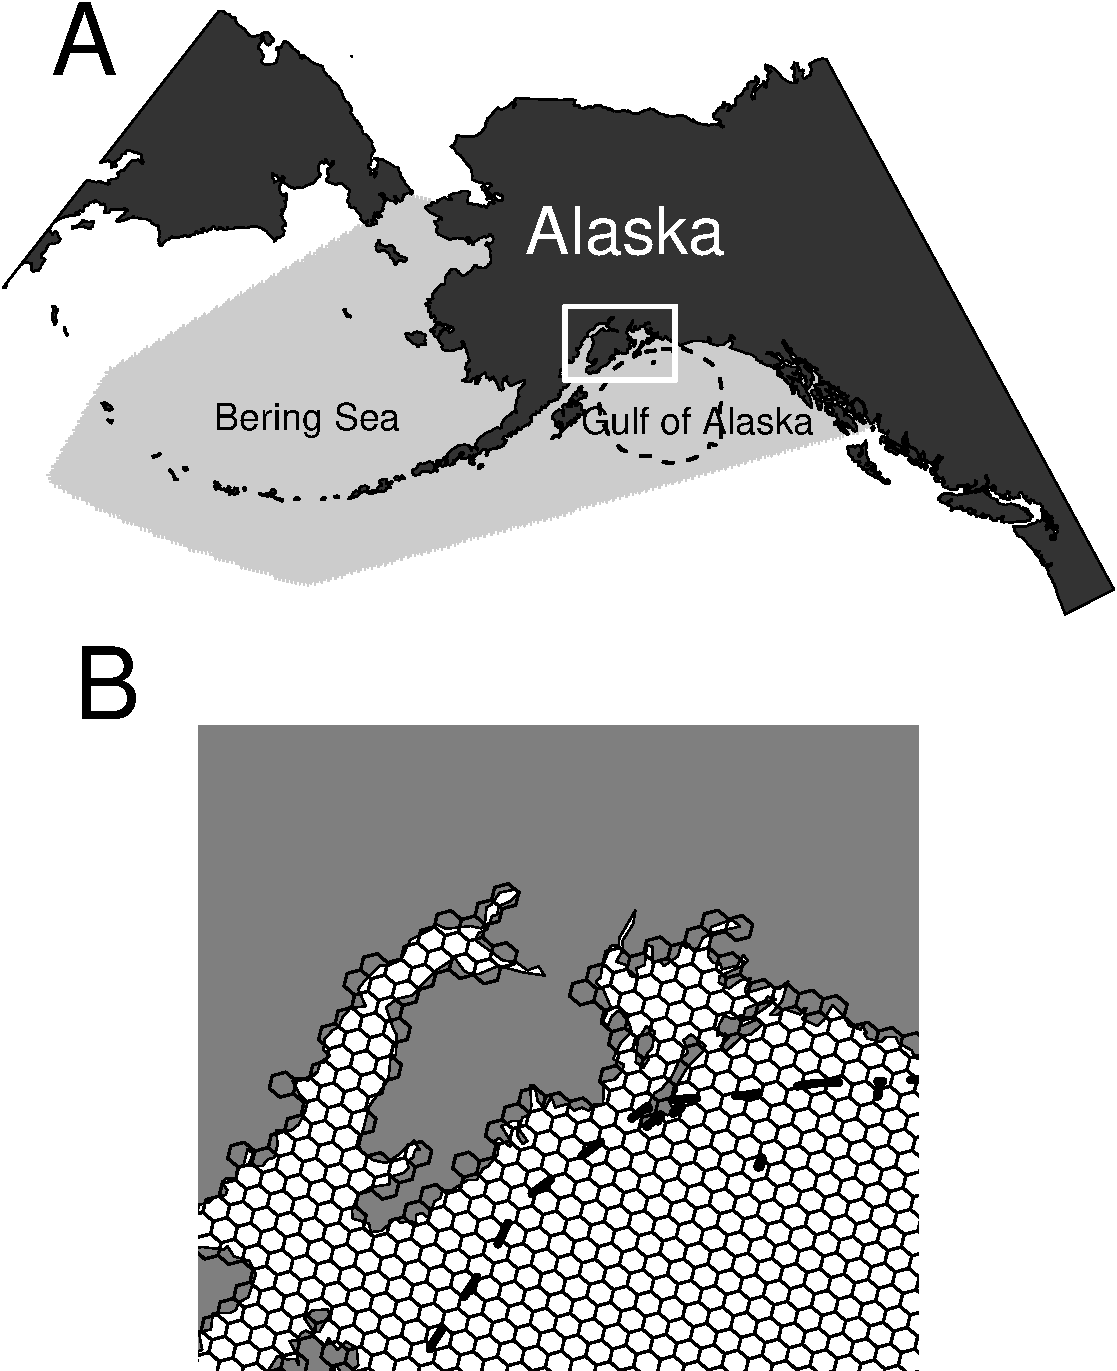
\includegraphics[width=.8\linewidth]{Fig-study_area}
  \end{center}
  \caption{Study area. A. Data were taken from the Bering Sea and Gulf of Alaska, shown by the light gray shade. The study area was gridded with 11,424 hexagons, but resolution is insufficient to plot them all. The white rectangular inset allows for more detail. The polygon with a dashed black line in the Gulf of Alaska is a Density Extent Area (DEA) used by the U.S. Navy. B.  A close-up of the white rectangular inset, showing hexagonal sample units, each of which was approximately 289 km$^{2}$.  \label{Fig-study_area}}         
\end{figure} 

\begin{figure}[H]
  \begin{center}
  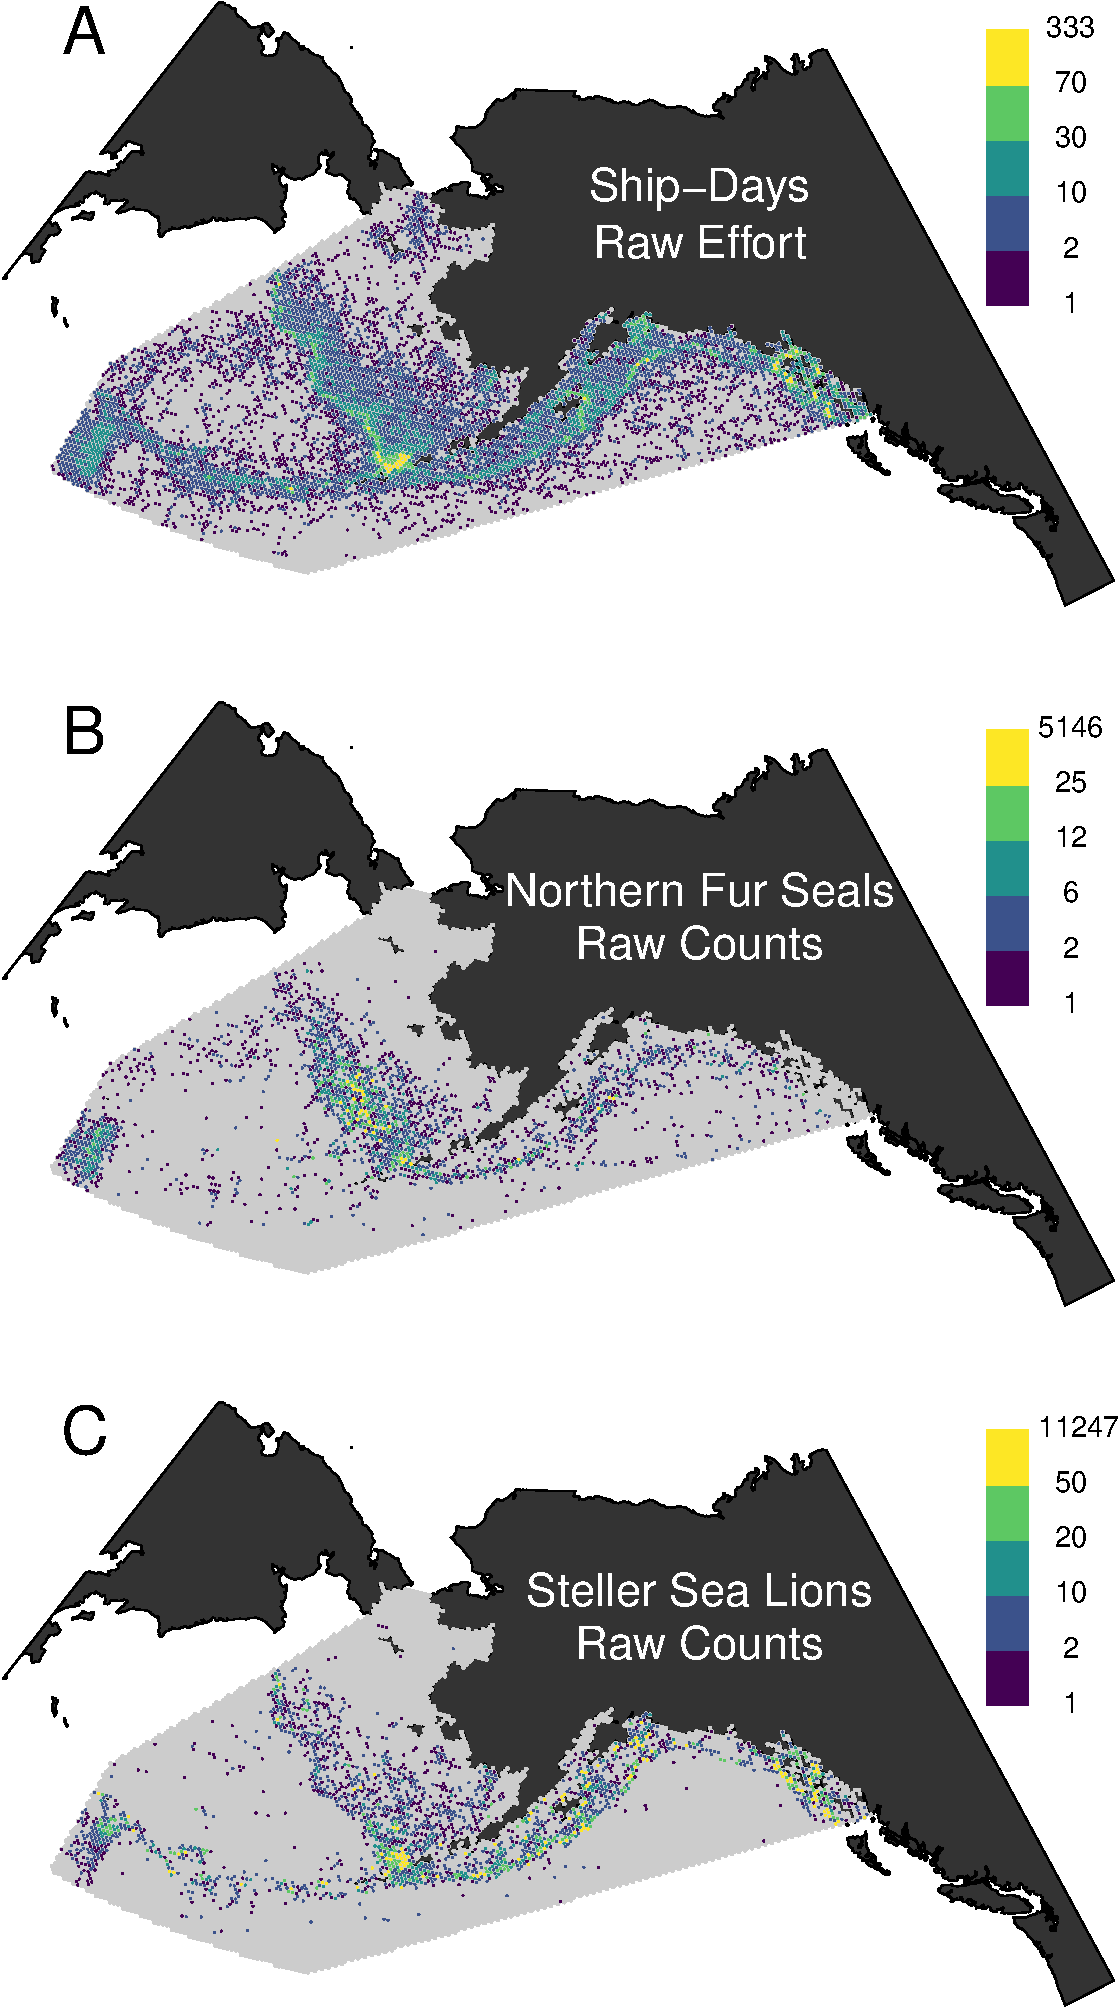
\includegraphics[width=.6\linewidth]{Fig-raw_data}
  \end{center}
  \caption{Raw data used for analyses. A. Ship-days in the study area. Hexagons without any ship days are contained in gray background. B. Northern fur seal counts in each hexagon, where zero counts are part of the gray background. C. Steller sea lion counts in each hexagon.  \label{Fig-raw_data}}         
\end{figure} 

\begin{figure}[H]
  \begin{center}
  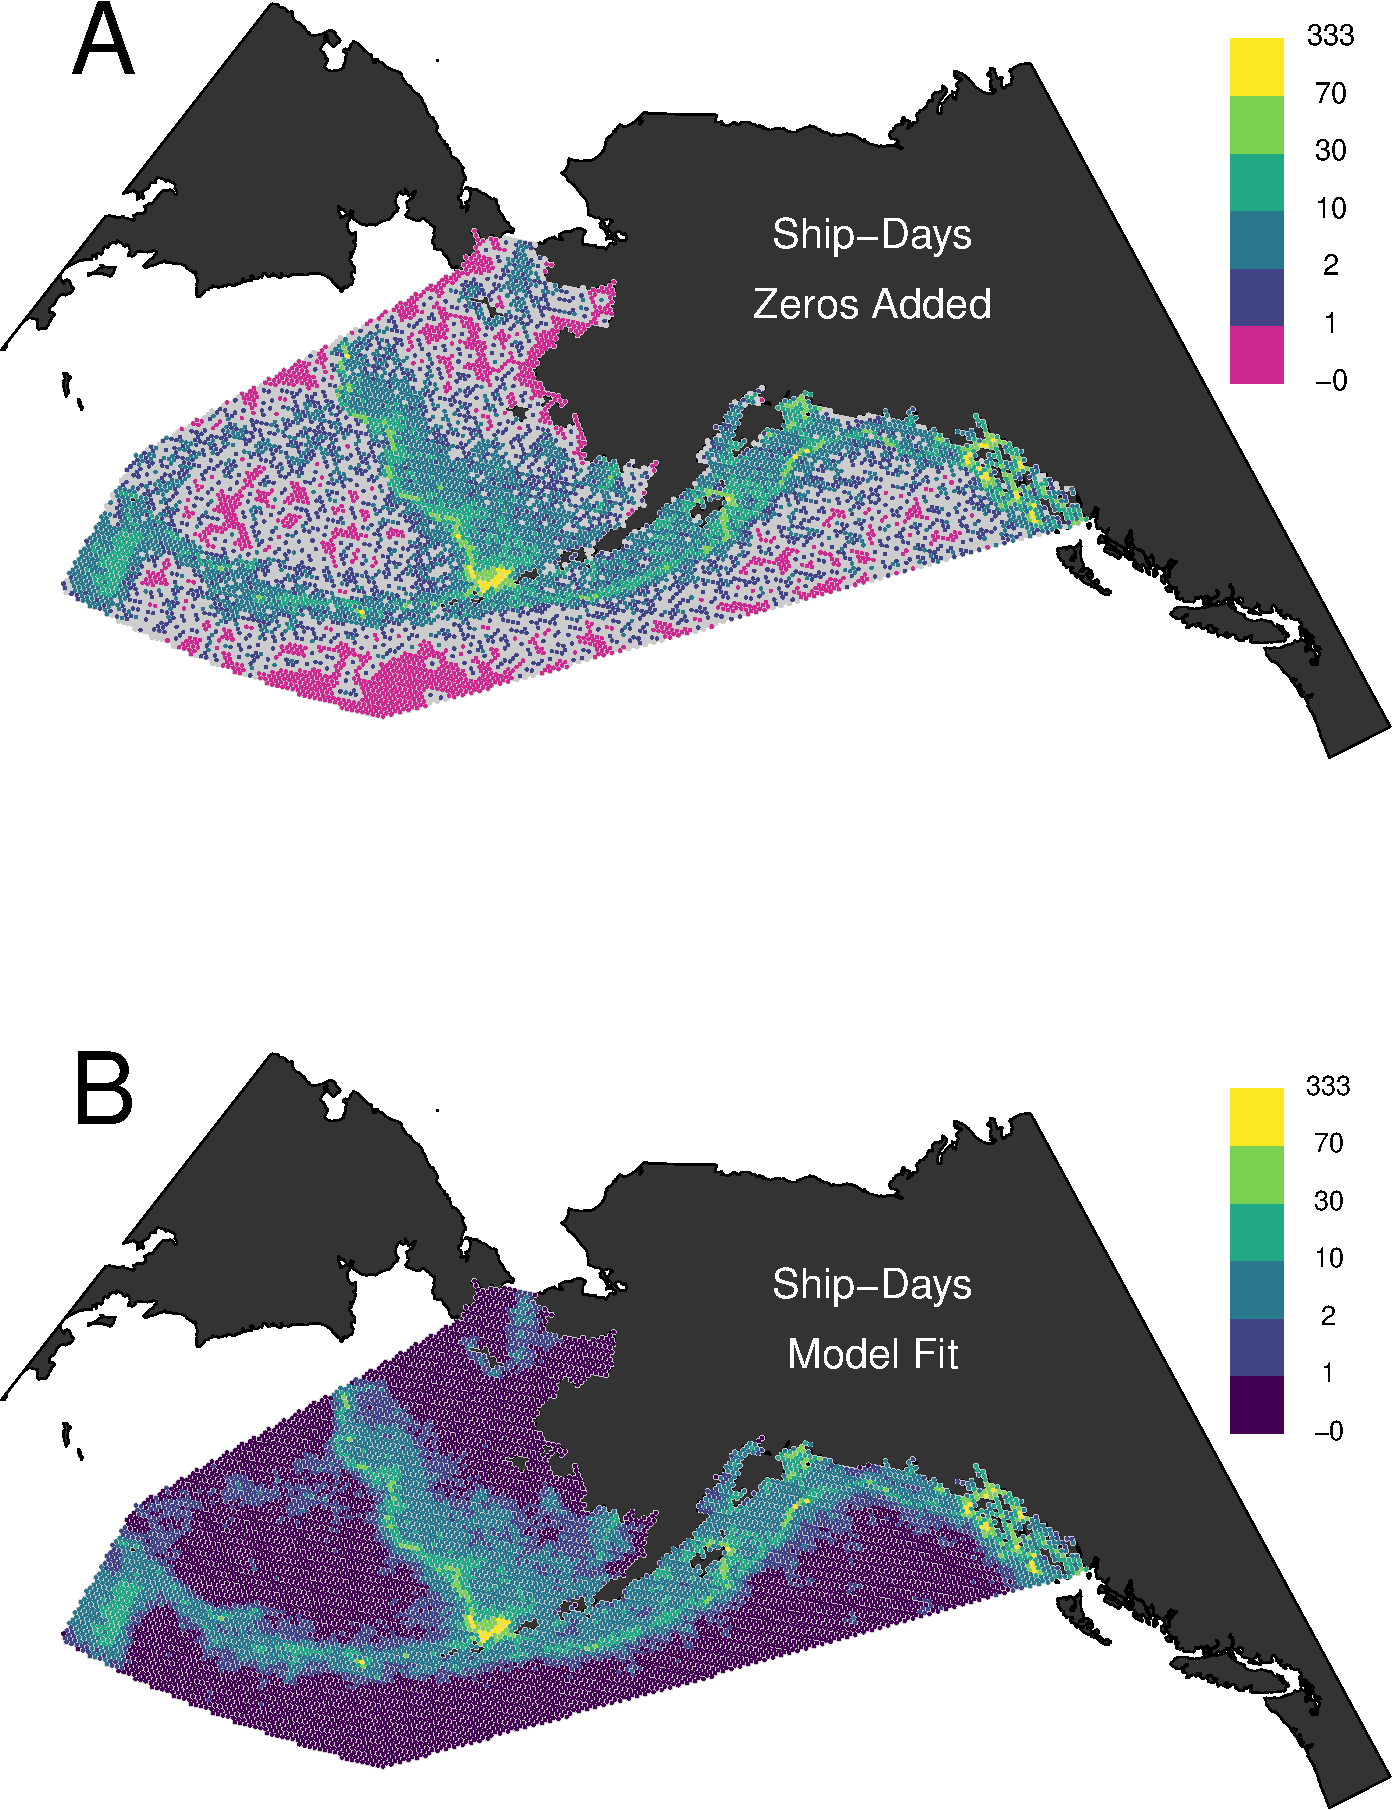
\includegraphics[width=.75\linewidth]{Fig-effort}
  \end{center}
  \caption{Effort data and model. A. Ship-days in the study area, where observed counts are the same as Figure~\ref{Fig-raw_data}A, except structural zeros have been added. Hexagons with a gray background were treated as missing data. B. Mode of the posterior distribution for ship-day for each hexagon using a negative binomial regression model with spatial random effects.  \label{Fig-Effort}}         
\end{figure} 

\begin{figure}[H]
  \begin{center}
  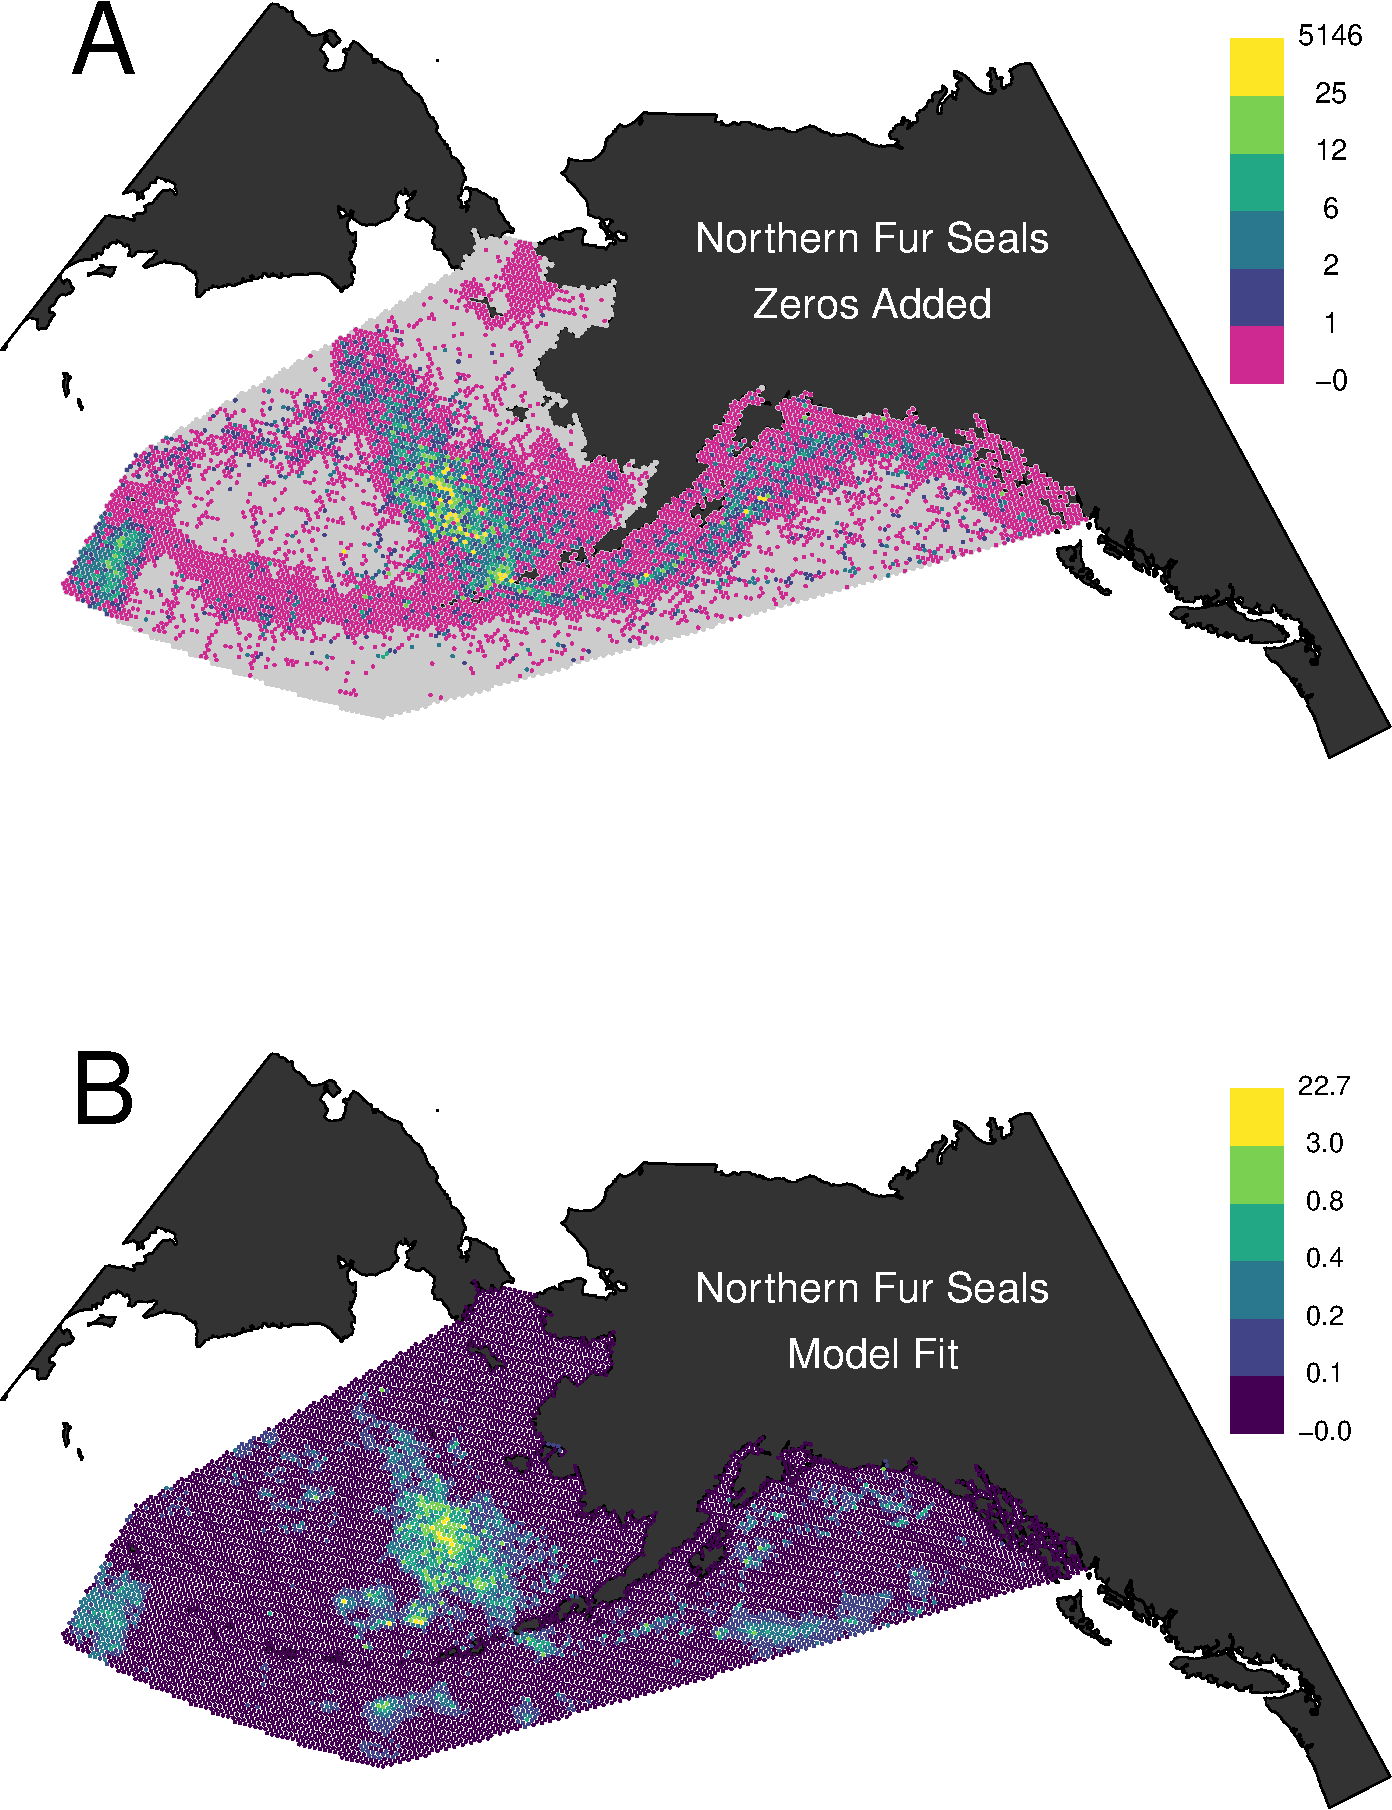
\includegraphics[width=.75\linewidth]{Fig-FurSealFit}
  \end{center}
  \caption{Northern fur seal data and model. A. Northern fur seal counts in the study area, where observed counts are the same as Figure~\ref{Fig-raw_data}B, except structural zeros have been added. Hexagons with a gray background were treated as missing data. B. Mode of the posterior distribution for northern fur seals per ship-day for each hexagon using a negative binomial regression model with spatial random effects.   \label{Fig-FurSealFit}}         
\end{figure} 

\begin{figure}[H]
  \begin{center}
  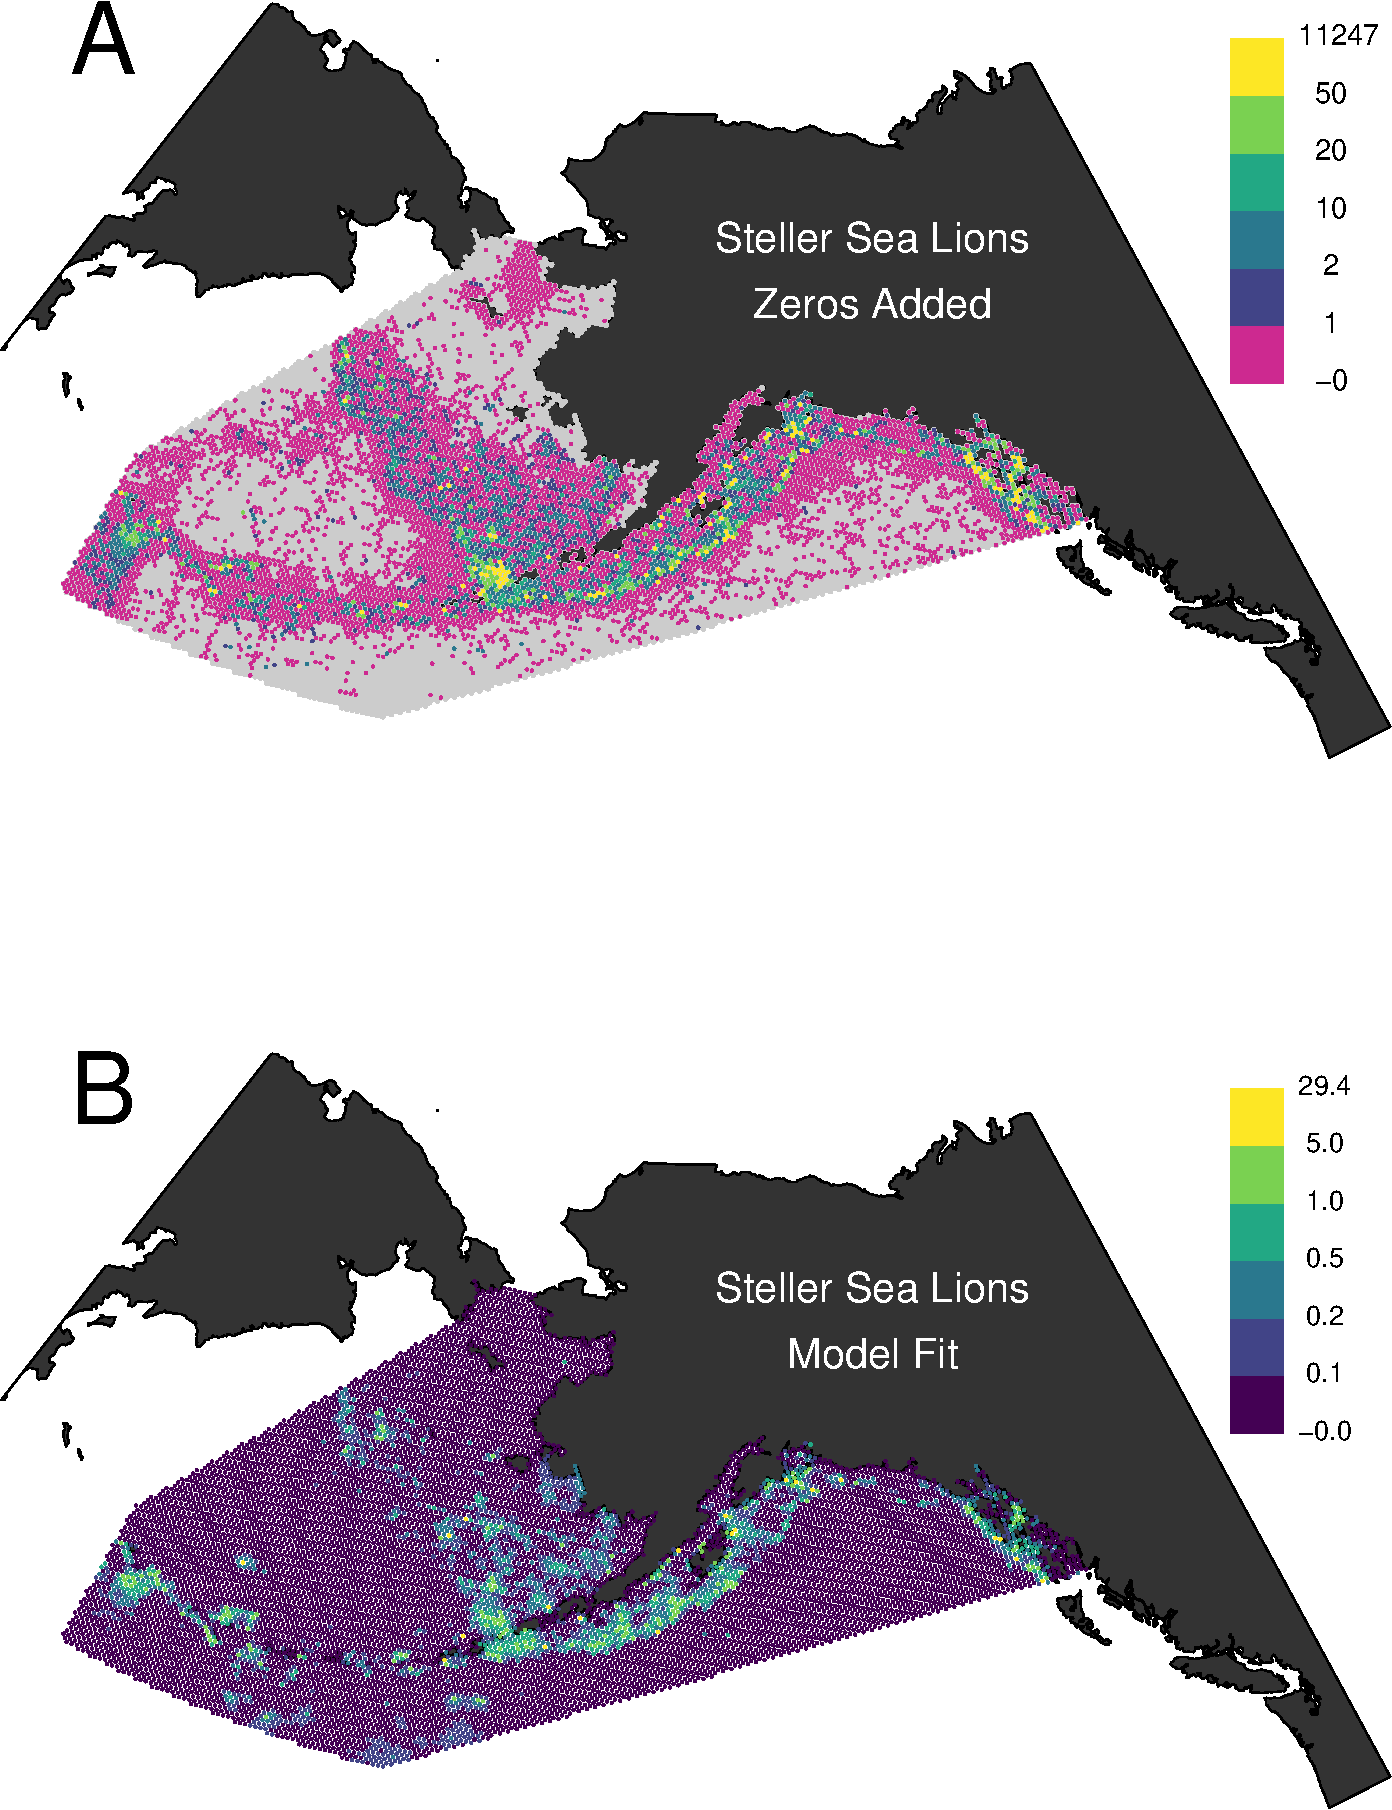
\includegraphics[width=.75\linewidth]{Fig-SeaLionFit}
  \end{center}
  \caption{Steller sea lion data and model. A. Steller sea lion counts in the study area, where observed counts are the same as Figure~\ref{Fig-raw_data}C, except structural zeros have been added. Hexagons with a gray background were treated as missing data. B. Mode of the posterior distribution for Steller sea lions per ship-day for each hexagon using a negative binomial regression model with spatial random effects.  \label{Fig-SeaLionFit}}         
\end{figure} 

\begin{figure}[H]
  \begin{center}
  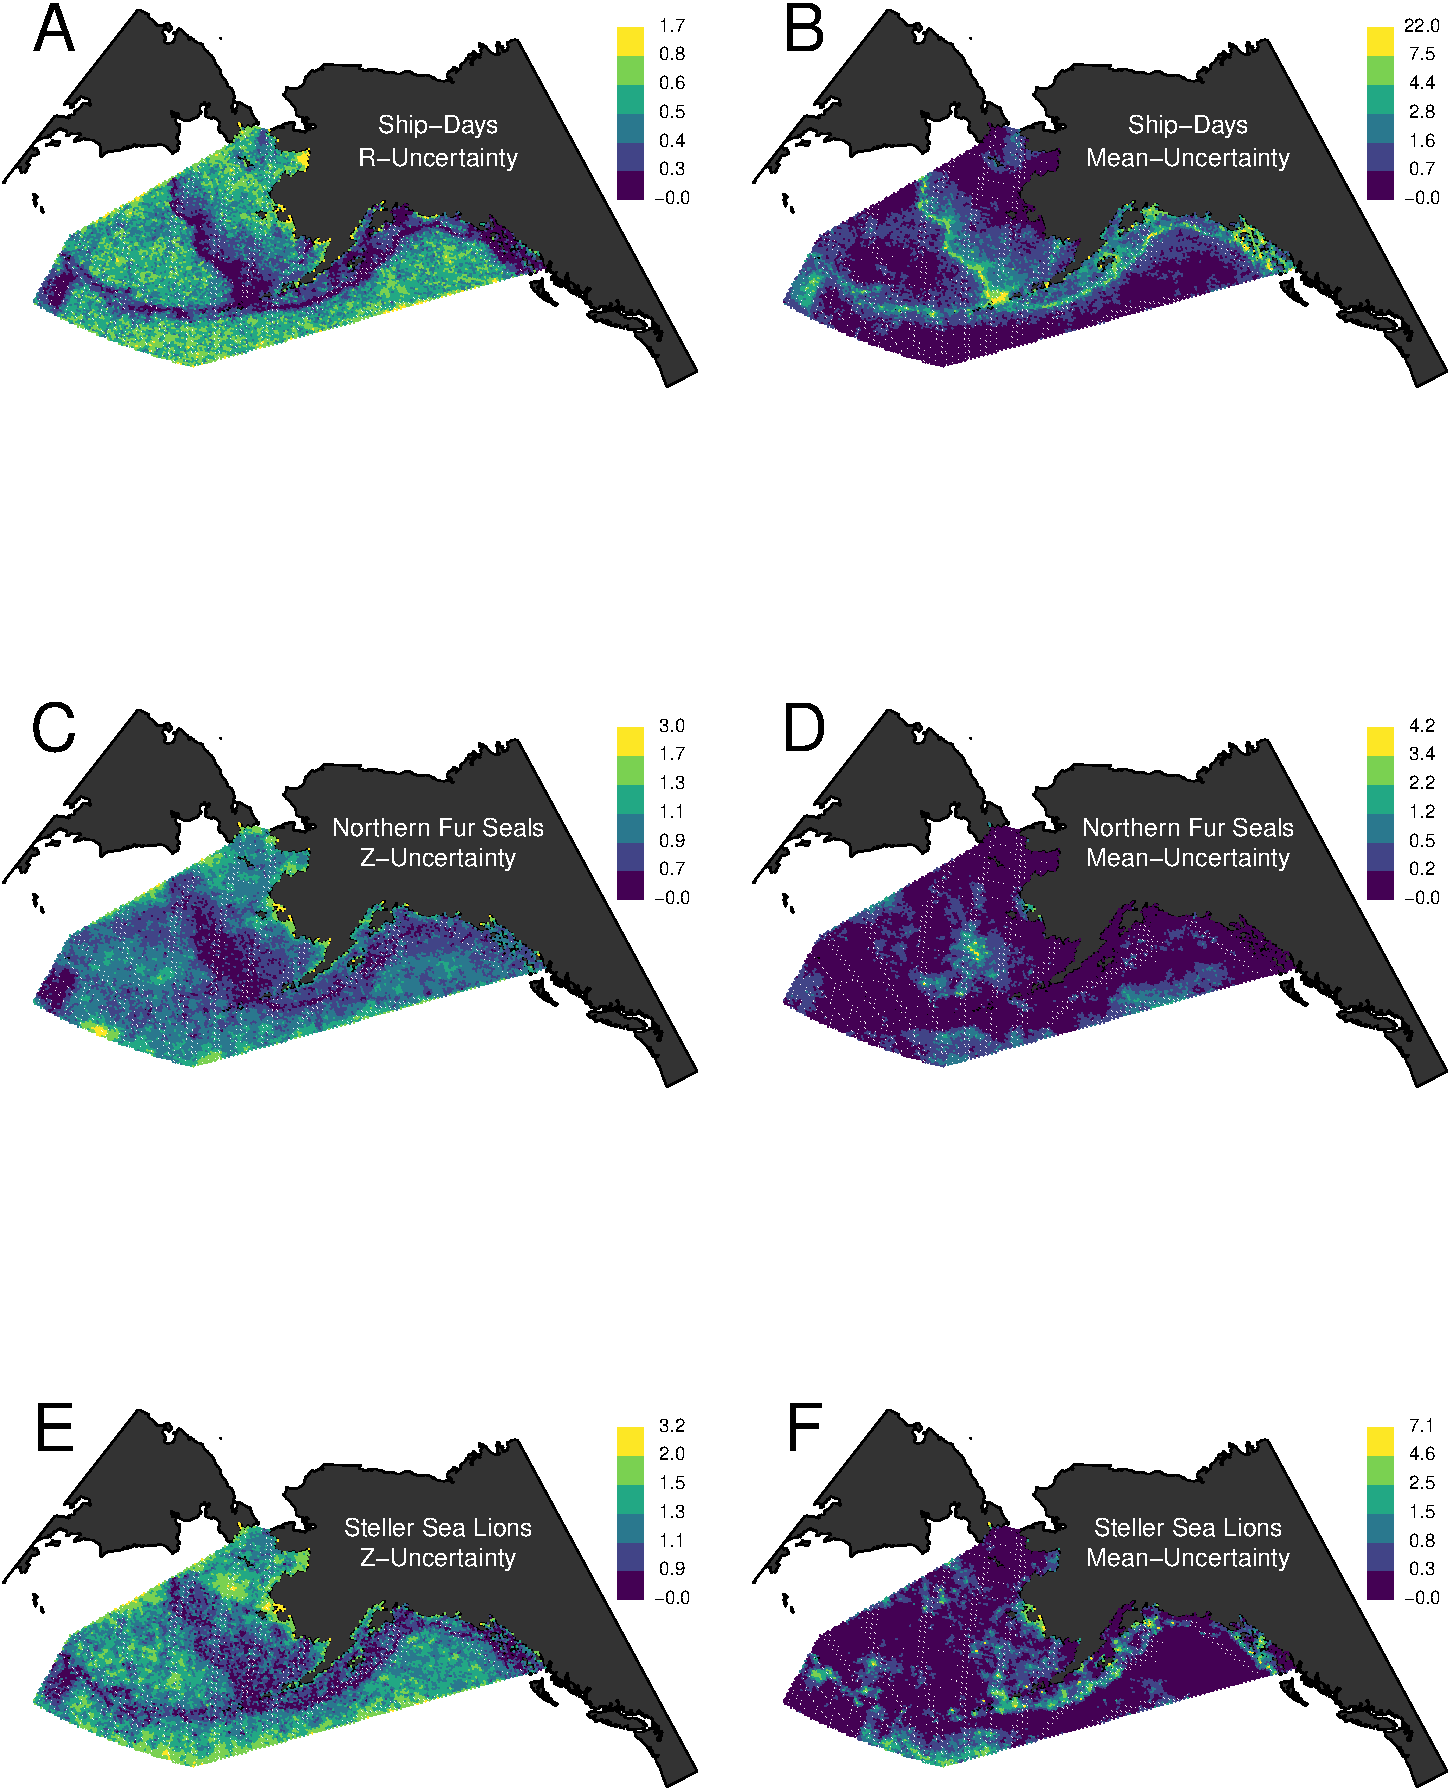
\includegraphics[width=.8\linewidth]{Fig-Uncertainty}
  \end{center}
  \caption{Model uncertainty. Standard deviation of each hexagon's posterior distribution  for: A) $R_{i}$ in $\br$ from Eq.~\eqref{eq:poireg}, B) $\exp(\alpha_{0} + R_{i})$ from Eq.~\eqref{eq:poireg}, C) $Z_{i}$ in $\bz$ from Eq.~\eqref{eq:poiregoff} for northern fur seals, D) $\exp(\beta_{0} + Z_{i})$ from Eq.~\eqref{eq:poiregoff} for northern fur seals, E) $Z_{i}$ in $\bz$ from Eq.~\eqref{eq:poiregoff} for Steller sea lions, D) $\exp(\beta_{0} + Z_{i})$ from Eq.~\eqref{eq:poiregoff} for Steller sea lions.
  \label{Fig-Uncertainty}}         
\end{figure} 

\begin{figure}[H]
  \begin{center}
  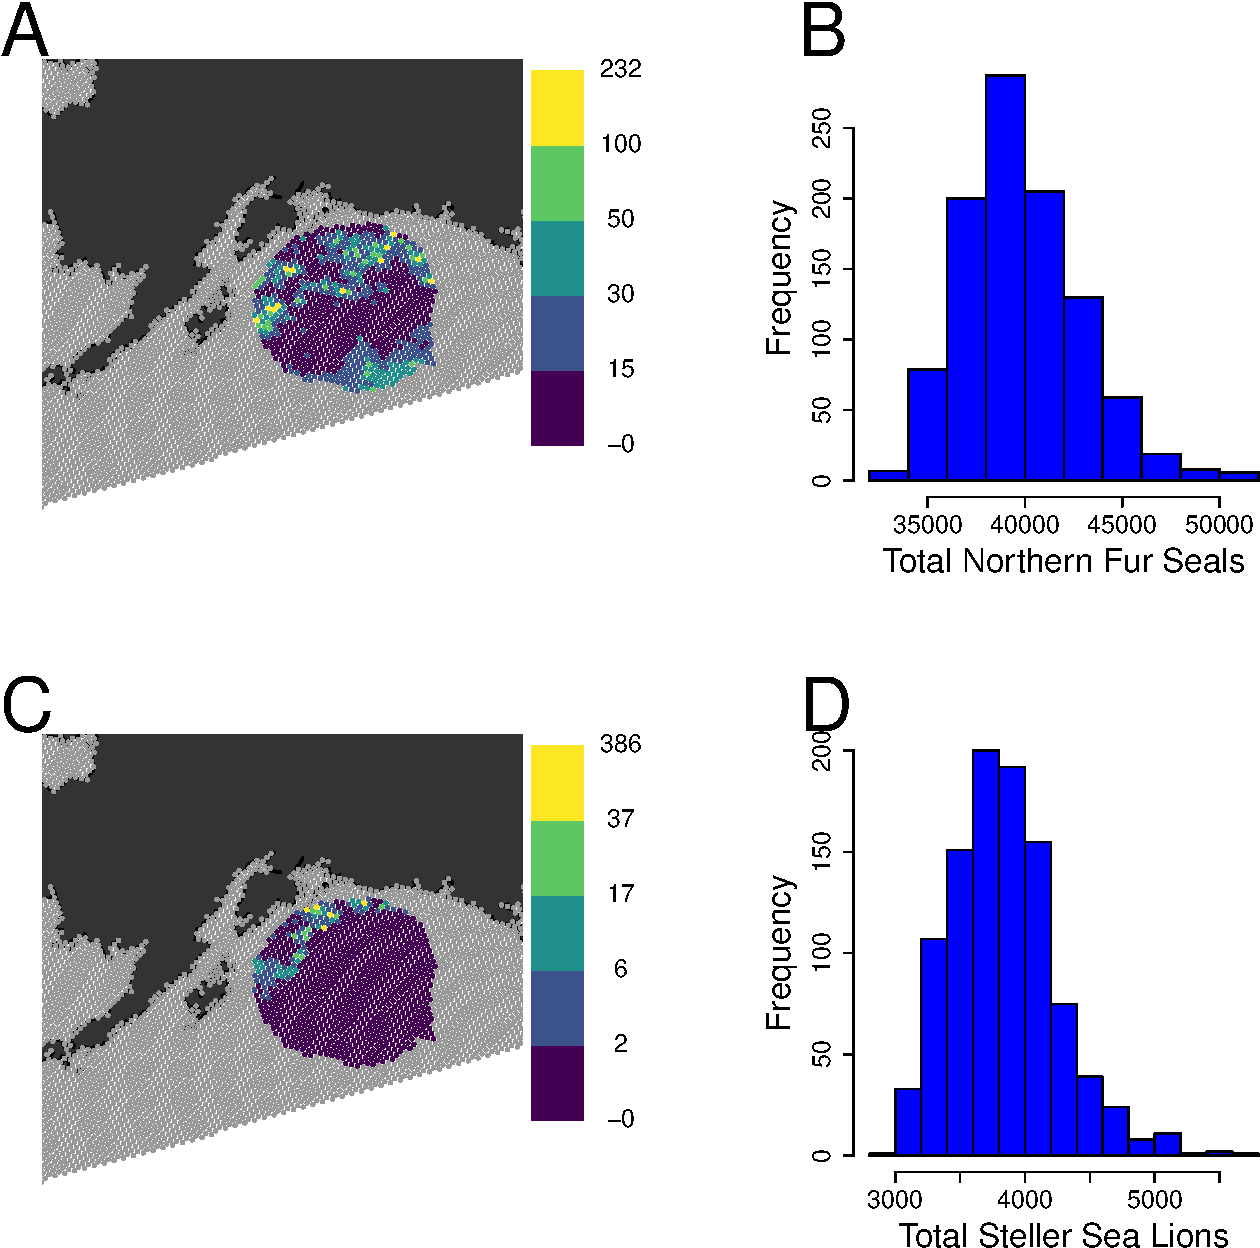
\includegraphics[width=.9\linewidth]{Fig-GOAabu}
  \end{center}
  \caption{Population estimates per hexagon in the Gulf of Alaska Density Extent Area (DEA). A. Map of mode of the posterior distribution for northern fur seal abundance in DEA. B. Histogram of MCMC sample from posterior distribution for total abundance of northern fur seals in DEA. C. Map of mode of the posterior distribution for Steller sea lions in DEA. D. Histogram of MCMC sample from posterior distribution for total abundance of Steller sea lions in DEA. \label{Fig-GOAabu}}         
\end{figure} 

\begin{figure}[H]
  \begin{center}
  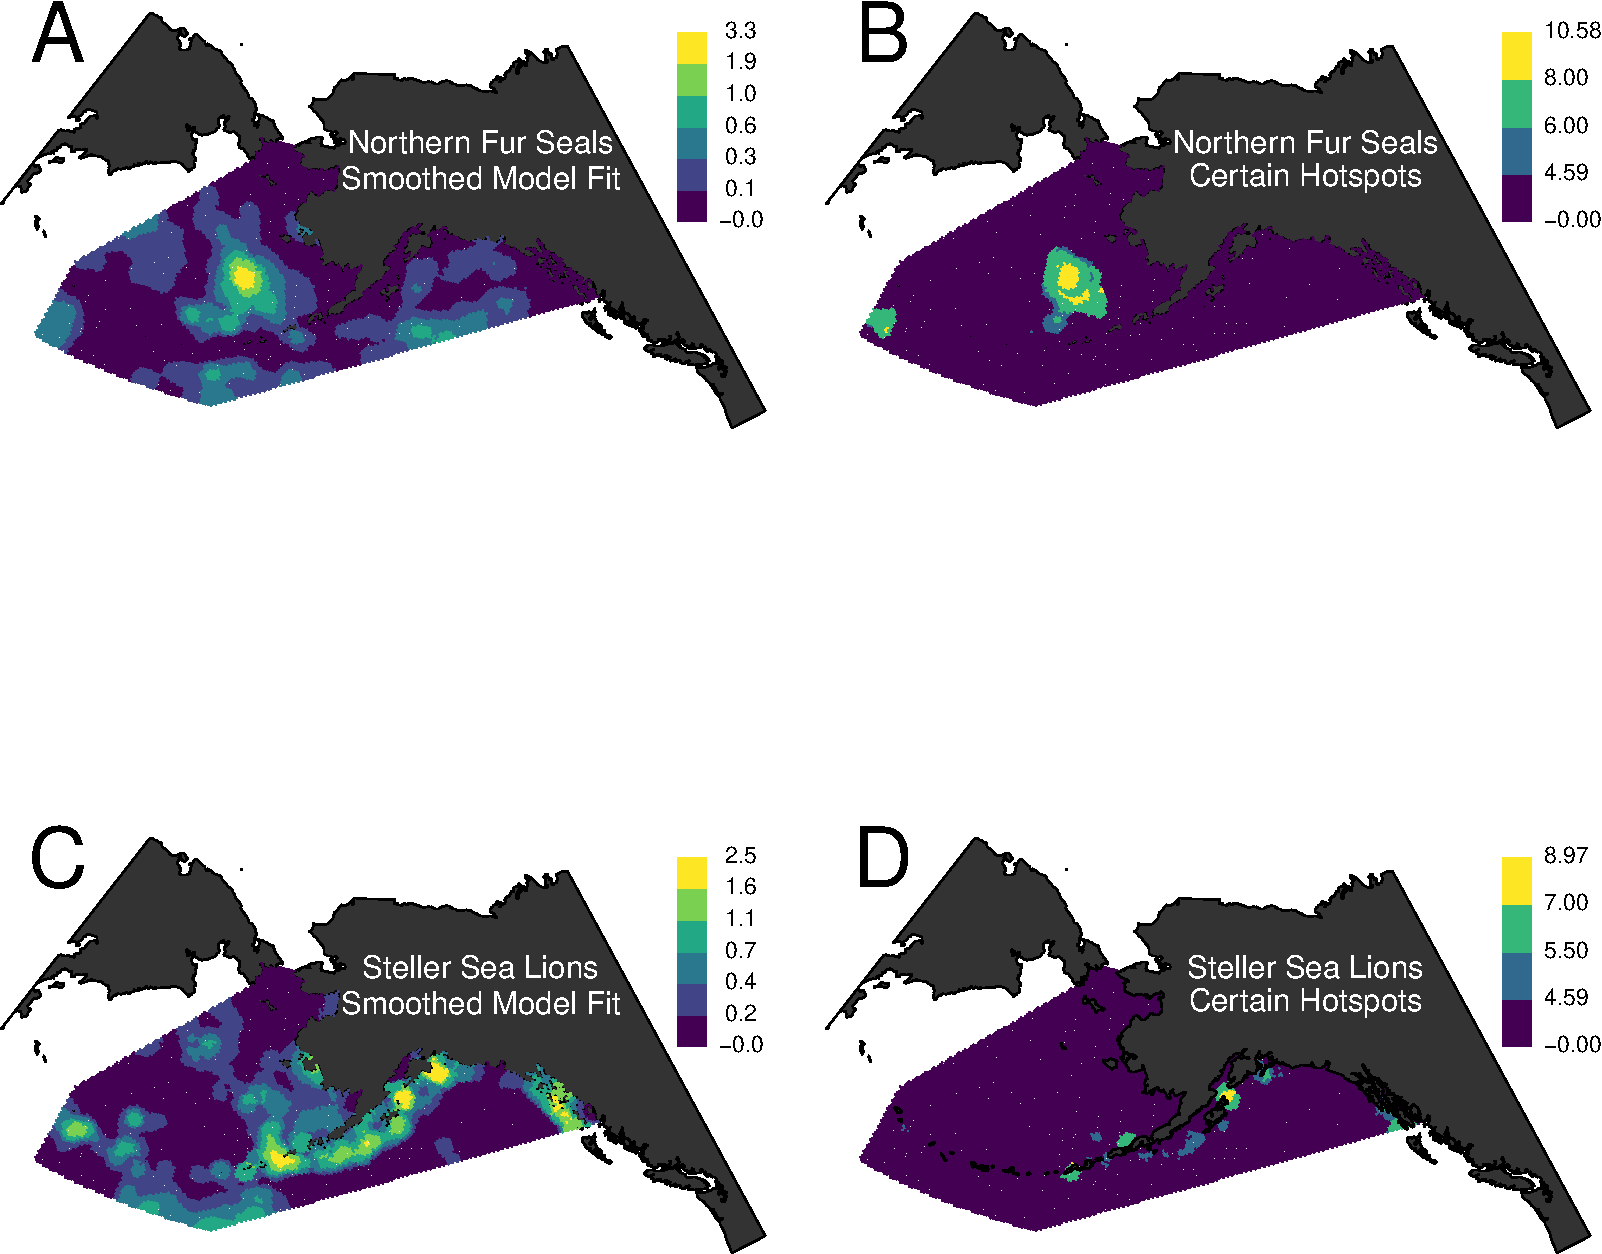
\includegraphics[width=1\linewidth]{Fig-SmooHotSpots}
  \end{center}
  \caption{Smoothing and Hotspots. A. Mode of each hexagon's posterior distribution after smoothing by averaging over 50 nearest neighbors for northern fur seals. B. Certain hotspots created by combining smoothing, thresholds, and uncertainty for northern fur seals. C. Mode of each hexagon's posterior distribution after smoothing by averaging over 50 nearest neighbors for Steller sea lions. D. Certain hotspots created by combining smoothing, thresholds, and uncertainty for Steller sea lions. \label{Fig-SmooHotSpots}}         
\end{figure} 



%%%%%%%%%%%%%%%%%%%%%%%%%%%%%%%%%%%%%%%%%%%%%%%%%%%%%%%%%%%%%%%%%%%%%%%%%%%%%%%%%%
%%%%%%%%%%%%%%%%%%%%%%%%%%%%%%%%%%%%%%%%%%%%%%%%%%%%%%%%%%%%%%%%%%%%%%%%%%%%%%%%%%
%%%%%%%%%%%            %%%%%%%    %%%%%%%%  %%%%%%%       %%%%%%%%%%%%%%%%%%%%%%%%
%%%%%%%%%%%  %%%%%%%%%%%%%%%%%  %  %%%%%%%  %%%%%%%  %%%%  %%%%%%%%%%%%%%%%%%%%%%%
%%%%%%%%%%%  %%%%%%%%%%%%%%%%%  %%  %%%%%%  %%%%%%%  %%%%%%  %%%%%%%%%%%%%%%%%%%%%
%%%%%%%%%%%  %%%%%%%%%%%%%%%%%  %%%  %%%%%  %%%%%%%  %%%%%%%   %%%%%%%%%%%%%%%%%%%
%%%%%%%%%%%            %%%%%%%  %%%%  %%%%  %%%%%%%  %%%%%%%%  %%%%%%%%%%%%%%%%%%%
%%%%%%%%%%%  %%%%%%%%%%%%%%%%%  %%%%%  %%%  %%%%%%%  %%%%%%%   %%%%%%%%%%%%%%%%%%%
%%%%%%%%%%%  %%%%%%%%%%%%%%%%%  %%%%%%  %%  %%%%%%%  %%%%%%  %%%%%%%%%%%%%%%%%%%%%
%%%%%%%%%%%  %%%%%%%%%%%%%%%%%  %%%%%%%  %  %%%%%%%  %%%%  %%%%%%%%%%%%%%%%%%%%%%%
%%%%%%%%%%%            %%%%%%%  %%%%%%%%    %%%%%%%       %%%%%%%%%%%%%%%%%%%%%%%%
%%%%%%%%%%%%%%%%%%%%%%%%%%%%%%%%%%%%%%%%%%%%%%%%%%%%%%%%%%%%%%%%%%%%%%%%%%%%%%%%%%
%%%%%%%%%%%%%%%%%%%%%%%%%%%%%%%%%%%%%%%%%%%%%%%%%%%%%%%%%%%%%%%%%%%%%%%%%%%%%%%%%%

\end{flushleft}
\end{spacing}
\end{document}


